\documentclass[12pt,a4paper]{report}

% ---------- Packages ----------
\usepackage[a4paper,margin=1in]{geometry}
\usepackage{graphicx}
\graphicspath{{figures/}}
\usepackage{booktabs}
\usepackage{tabularx}
\usepackage{array}
\usepackage{amsmath}
\usepackage{amssymb}
\usepackage{float}
\usepackage{subcaption}
\usepackage{xcolor}
\usepackage{listings}
\usepackage{enumitem}
\usepackage{longtable}
\usepackage{multirow}
\usepackage{caption}
\usepackage{placeins}
\usepackage{microtype}
\usepackage[colorlinks=true,linkcolor=blue!50!black,citecolor=blue!50!black,urlcolor=blue!50!black]{hyperref}

% Zero-width break point (no inserted hyphen), used inside \texttt paths.
\newcommand{\pbrk}{\discretionary{}{}{}}
\usepackage{setspace}
\onehalfspacing

\captionsetup{font=small,labelfont=bf}

\lstset{
  basicstyle=\ttfamily\small,
  breaklines=true,
  frame=single,
  columns=fullflexible,
  backgroundcolor=\color{gray!8}
}

\title{
  \vspace{-2cm}
  \Huge\textbf{CrisisSense} \\[0.4cm]
  \Large Crisis Language Detection Using NLP \\[0.2cm]
  \large A Comparative Study of Character-Level TF-IDF and Transformer-Based\\
  Text Classification for Three-Class Crisis-Language Detection
}
\author{CrisisSense Project}
\date{September 2026}

\begin{document}

\begin{titlepage}
\centering
\vspace*{2cm}
{\Huge\textbf{CrisisSense}}\\[0.5cm]
{\Large Crisis Language Detection Using NLP}\\[1.5cm]
{\large\textbf{A Comparative Study of Character-Level TF-IDF and Transformer-Based}}\\
{\large\textbf{Text Classification for Three-Class Crisis-Language Detection}}\\[3cm]
{\large Final Academic Project Report}\\[1cm]
{\large Natural Language Processing Laboratory}\\[3cm]
{\large September 2026}\\
\vfill
\textit{This system performs text classification only. It is not a clinical diagnostic tool and does not assess suicide risk.}
\end{titlepage}

\pagenumbering{roman}
\tableofcontents
\listoffigures
\listoftables
\clearpage
\pagenumbering{arabic}

\chapter*{Abstract}
\addcontentsline{toc}{chapter}{Abstract}

Crisis-related language on text platforms is frequently expressed indirectly, which makes automatic detection difficult for systems that rely on explicit keyword matching. This report presents CrisisSense, a frozen three-class text-classification system that labels submitted text as \texttt{no\_crisis}, \texttt{implicit\_crisis}, or \texttt{explicit\_crisis}. CrisisSense runs two independently trained models on each input --- a character-level TF-IDF representation with a Logistic Regression classifier, and a locally hosted BERT sequence classifier --- and displays both predictions side by side without combining them into an ensemble.

Both models are evaluated on the same frozen 195-row test split, drawn from a 1{,}294-row dataset partitioned into 905 training, 194 validation, and 195 test rows. On this shared test set, BERT attains higher overall accuracy (76.92\% vs. 71.28\%) and macro-F1 (74.66\% vs. 69.62\%) than the TF-IDF baseline. However, this overall advantage does not extend uniformly to every class: TF-IDF with Logistic Regression achieves a marginally higher F1 score on the implicit-crisis class specifically (67.92\% vs. 67.33\%), a category in which crisis intent is not stated directly and both models struggle relative to their explicit-crisis performance. Confidence and calibration analysis further shows that BERT's mean selected-class confidence (94.60\%) is substantially higher than TF-IDF's (55.74\%), yet BERT's Expected Calibration Error (0.177) is also higher than TF-IDF's (0.155), indicating that BERT's higher confidence does not correspond to proportionally higher reliability. The two models agree on 75.9\% of test samples (148/195) and disagree on the remaining 24.1\%, and agreement is shown not to be a proxy for correctness.

This report documents the current frozen CrisisSense system as implemented and deployed: its dataset, its TF-IDF and BERT pipelines, its FastAPI backend and static frontend, its evaluation protocol, and its quantitative results, including per-class performance, confusion matrices, confidence distributions, calibration behavior, and an aggregate error analysis drawn from the shared test-set predictions. CrisisSense classifies crisis-related language in text; it does not diagnose individuals, assess suicide risk, or substitute for professional clinical judgment, and all interpretations in this report are scoped to the 195-sample frozen evaluation set on which they were measured.

\chapter{Introduction}

\section{Background}

Text-based platforms increasingly serve as spaces where individuals express psychological distress, and crisis-related language on these platforms rarely takes a single, uniform shape. Some statements name crisis intent directly; others communicate the same underlying meaning indirectly, through metaphor, understatement, or contextual cues that require inference rather than lexical matching. A detection system built only on keyword or lexicon matching will reliably catch the former and largely miss the latter, while a system with no lexical grounding at all may over-generalize from superficial similarity. This tension between direct and indirect expression motivates CrisisSense, which treats crisis-language detection as a three-class text-classification problem and studies how two structurally different models --- a sparse, character-level lexical model and a contextual transformer --- perform on the same task and the same data.

\section{Problem Statement}

Given a short piece of submitted text, the task addressed by CrisisSense is to assign one of three labels:

\begin{itemize}[nosep]
  \item \textbf{Class 0 --- \texttt{no\_crisis}}: text that does not indicate crisis-related language under the current classification scheme.
  \item \textbf{Class 1 --- \texttt{implicit\_crisis}}: crisis-related meaning expressed indirectly rather than as a direct statement.
  \item \textbf{Class 2 --- \texttt{explicit\_crisis}}: crisis-related language expressed directly.
\end{itemize}

This is a single-label, three-class classification problem over free text. It is explicitly \emph{not} a four-class or severity-graded problem, not a clinical risk-assessment task, and not a generative or conversational task: the system produces a class label and a probability distribution over the three classes, nothing more.

\section{Motivation}

Implicit crisis language is the harder and arguably more consequential case: it is the category most likely to be missed by naive keyword filters, yet it is also the category with the fewest unambiguous lexical cues to exploit. Comparing a lexical, character-level model against a contextual transformer model on the same frozen test set makes it possible to ask a concrete empirical question --- does additional contextual modeling capacity actually help on the implicit-crisis class specifically, or only on the classification task in aggregate --- rather than relying on the intuition that "bigger models are strictly better."

\section{Objectives}

The objectives of this project, as reflected in the current frozen system, are to:

\begin{enumerate}[nosep]
  \item Build a reproducible, frozen three-class dataset split (train/validation/test) with verified class balance and no duplicate or overlapping rows.
  \item Train and freeze a character-level TF-IDF plus Logistic Regression baseline as a lexical, computationally lightweight classifier.
  \item Load and evaluate a BERT sequence-classification model as a contextual counterpart, without retraining it as part of the deployed system.
  \item Evaluate both frozen models on an identical held-out test set and report accuracy, macro-averaged precision/recall/F1, per-class F1, confidence statistics, calibration error, and inter-model agreement.
  \item Serve both models independently, side by side, through a single FastAPI backend and a static frontend, without combining their outputs into an ensemble.
\end{enumerate}

\section{Contributions}

This report's contributions are:

\begin{enumerate}[nosep]
  \item A documented, reproducible three-class crisis-language dataset split (905/194/195 rows) with a verified provenance chain and zero cross-split duplication.
  \item A fully specified TF-IDF + Logistic Regression pipeline (character n-grams, \texttt{char\_wb} analyzer, frozen hyperparameters) evaluated end to end on the shared test set.
  \item A fully specified BERT sequence-classification pipeline (12-layer, 768-hidden, 12-head, 3-label \texttt{BertForSequenceClassification}) evaluated as a frozen inference-only artifact on the same test set.
  \item A side-by-side comparison of the two models covering overall metrics, per-class metrics, confusion matrices, confidence distributions, Expected Calibration Error, and model agreement/disagreement.
  \item An explicit boundary statement distinguishing the currently deployed three-class system from historical four-class, severity-graded, and Word2Vec-based research material retained elsewhere in the repository but not used at runtime.
\end{enumerate}

\section{Scope}

The scope of this report is limited to the currently deployed CrisisSense system: the static frontend (\texttt{index.html}), the FastAPI backend (\texttt{backend/\pbrk app.py}), the frozen dataset splits under \texttt{data/\pbrk final\_\pbrk datasets/\pbrk splits/\pbrk }, the frozen TF-IDF/Logistic Regression and BERT artifacts, and the evaluation outputs under \texttt{results/\pbrk model\_\pbrk comparison/\pbrk }. The repository additionally contains historical four-class research material (alternate annotation schemes, an unused Word2Vec path, and earlier BERT training modules) that predates the current system; this material is explicitly out of scope and is not used by any component described in this report. CrisisSense is a research and coursework artifact for crisis-related text classification; it is not a medical device, does not diagnose individuals, and does not assess suicide risk.

\chapter{Related Work}

\section{Crisis- and Suicide-Related Language Detection}

Automatic detection of crisis- and suicide-related language is a recognized application area within applied NLP, typically framed as a text-classification or risk-stratification problem over social-media posts, forum text, or clinical notes. A recurring difficulty in this literature is that crisis intent is often not stated in an unambiguous, keyword-matchable form; language can convey the same underlying state through indirection, metaphor, or understatement. This motivates treating implicit and explicit expression as distinct classes rather than collapsing them into a single binary crisis/no-crisis label, which is the design choice CrisisSense makes with its three-class scheme.

\section{Traditional NLP Classification}

Before the widespread adoption of pretrained transformer encoders, text classification was dominated by sparse, feature-based pipelines: a document is mapped to a high-dimensional numeric vector (bag-of-words, n-gram counts, or TF-IDF weights), and a linear or shallow classifier is fit on top of that vector. These pipelines remain competitive baselines because they are inexpensive to train, fast at inference time, and behave predictably on out-of-distribution or noisy text, which is a relevant property for short, informally written crisis-related messages.

\section{TF-IDF and Linear Models}

Term Frequency--Inverse Document Frequency (TF-IDF) weighting~\cite{sparckjones1972statistical} scores a term within a document in proportion to how often it appears in that document and in inverse proportion to how common it is across the whole corpus, so that terms that are frequent everywhere contribute little discriminative signal. Logistic Regression~\cite{cox1958regression} is the standard linear classifier paired with TF-IDF features, mapping the resulting sparse feature vector to class probabilities through a softmax over a linear score. Character-level n-gram variants of TF-IDF (as opposed to word-level n-grams) are particularly relevant for informal, misspelled, or non-standard text, since they degrade gracefully under spelling variation and do not require a fixed vocabulary of whole words.

\section{Transformer-Based Text Classification}

The Transformer architecture~\cite{vaswani2017attention} replaced recurrence with self-attention, allowing every token in a sequence to attend directly to every other token. This architecture underlies the current generation of pretrained language models used for text classification, in which a large encoder is pretrained on unlabeled text and then fine-tuned (or, as in the present system, previously fine-tuned and subsequently frozen) for a downstream classification task by attaching a linear classification head to a pooled sequence representation.

\section{BERT}

BERT~\cite{devlin2019bert} is a bidirectional Transformer encoder pretrained with a masked-language-modeling objective, producing contextual token representations that condition on both left and right context simultaneously. \texttt{BertForSequenceClassification}, the architecture used by the CrisisSense BERT artifact, attaches a linear classification head to BERT's pooled output and is a standard configuration for sequence-level classification tasks such as sentiment analysis, topic classification, and --- as in this report --- crisis-language classification. The publicly available implementation used here is provided through the Hugging Face Transformers library~\cite{wolf2020transformers} and runs on PyTorch~\cite{paszke2019pytorch}.

\section{Comparison of Traditional and Transformer Approaches}

Contextual transformer models are generally expected to outperform sparse lexical baselines on tasks that require disambiguating meaning from context, since self-attention can, in principle, capture the kind of indirection and dependency structure that a bag-of-character-n-grams representation cannot. However, this expected advantage is not guaranteed to be uniform across all classes of a task: a model can improve overall accuracy while leaving a specific, harder subclass unchanged or only marginally improved, particularly when that subclass is defined by pragmatic or contextual indirection (as implicit crisis language is) rather than by surface lexical variation alone. Neural classifiers, including fine-tuned transformers, have also been repeatedly shown to be poorly calibrated: their softmax confidence does not reliably track the true probability of correctness~\cite{guo2017calibration,naeini2015obtaining}. This is directly relevant to interpreting CrisisSense's results, since the BERT model in this system produces markedly higher confidence scores than the TF-IDF model without a proportional improvement in calibration.

\section{Research Gap and Motivation}

Much of the applied literature on crisis-language detection reports a single model's aggregate accuracy without separating overall performance from class-specific performance, and without jointly reporting confidence, calibration, and inter-model agreement as distinct axes of evaluation. CrisisSense is positioned to address this gap directly for its own dataset: it evaluates two independently trained models of different representational character (sparse lexical vs. contextual transformer) on an identical frozen test set, and reports overall metrics, per-class metrics, confidence, calibration, and agreement as separate, non-interchangeable quantities, consistent with the general finding that high confidence does not imply high accuracy and that overall accuracy does not imply uniform per-class advantage.

\chapter{Dataset}
\label{ch:dataset}

\section{Current Dataset}

CrisisSense's frozen split copies live under \texttt{data/\pbrk final\_\pbrk datasets/\pbrk splits/\pbrk } (\texttt{train.csv}, \texttt{validation.csv}, \texttt{test.csv}). Each row provides a \texttt{content} field (the input text) and a \texttt{label} field (the three-class target, 0/1/2), alongside \texttt{row\_index}, \texttt{url}, \texttt{class\_name}, and \texttt{split} columns. These three files are explicit, byte-preserved copies of the authoritative split file \texttt{experiments/\pbrk tfidf\_\pbrk baseline/\pbrk results/\pbrk data\_\pbrk split.csv}, filtered by its existing \texttt{split} column; no resampling, shuffling, or re-partitioning was performed in producing the copies, and row order, text, and labels are unchanged from the source. The split-provenance record (\texttt{data/\pbrk final\_\pbrk datasets/\pbrk splits/\pbrk README.md}) documents this chain and states that if the copies ever disagree with the source file, the source file is authoritative.

\section{Label Definitions}

Table~\ref{tab:class-defs} gives the current three-class label scheme, including the mapping from the dataset's original ordinal \texttt{severity} field (0--6) into the collapsed three-class \texttt{label} field used by both models.

\begin{table}[H]
\centering
\caption{Current class definitions and their construction from the original severity scale.}
\label{tab:class-defs}
\begin{tabular}{clp{7.2cm}}
\toprule
\textbf{ID} & \textbf{Class} & \textbf{Meaning} \\
\midrule
0 & \texttt{no\_crisis} & Text that does not indicate crisis-related language under the current scheme. Constructed from original \texttt{severity} = 0. \\
1 & \texttt{implicit\_crisis} & Crisis-related meaning expressed indirectly rather than as a direct statement. Constructed from original \texttt{severity} = 1. \\
2 & \texttt{explicit\_crisis} & Crisis-related language expressed directly. Constructed from original \texttt{severity} $\in \{2,\dots,6\}$. \\
\bottomrule
\end{tabular}
\end{table}

Detailed provenance of the original annotation process that produced the \texttt{severity} values is not verifiable from the current runtime implementation alone; the repository's historical documentation describes a separate four-class annotation design, which is not the label definition used by the currently deployed models and must not be read as such.

\section{Dataset Split}

The dataset is partitioned into training, validation, and test splits using a stratified 70/15/15 split (seed 42), as recorded in \texttt{models/\pbrk tfidf\_\pbrk logistic\_\pbrk regression/\pbrk config.json}. Table~\ref{tab:split-sizes} gives the resulting row counts.

\begin{table}[H]
\centering
\caption{Frozen dataset split sizes.}
\label{tab:split-sizes}
\begin{tabular}{lrr}
\toprule
\textbf{Split} & \textbf{Path} & \textbf{Rows} \\
\midrule
Train      & \texttt{data/\pbrk final\_\pbrk datasets/\pbrk splits/\pbrk train.csv}      & 905 \\
Validation & \texttt{data/\pbrk final\_\pbrk datasets/\pbrk splits/\pbrk validation.csv} & 194 \\
Test       & \texttt{data/\pbrk final\_\pbrk datasets/\pbrk splits/\pbrk test.csv}       & 195 \\
\midrule
\textbf{Total} & & \textbf{1{,}294} \\
\bottomrule
\end{tabular}
\end{table}

Both the TF-IDF/Logistic Regression model and the BERT model are evaluated on exactly the same 195-row \texttt{test.csv}; the results in Chapter~\ref{ch:results} are directly comparable because they share this identical evaluation set.

\section{Class Distribution}

Table~\ref{tab:class-dist} reports the per-class row counts within each split.

\begin{table}[H]
\centering
\caption{Class distribution across the frozen splits.}
\label{tab:class-dist}
\begin{tabular}{lrrrr}
\toprule
\textbf{Split} & \textbf{No Crisis (0)} & \textbf{Implicit Crisis (1)} & \textbf{Explicit Crisis (2)} & \textbf{Total} \\
\midrule
Train      & 245 & 227 & 433 & 905 \\
Validation & 53  & 48  & 93  & 194 \\
Test       & 53  & 49  & 93  & 195 \\
\midrule
\textbf{Total} & \textbf{351} & \textbf{324} & \textbf{619} & \textbf{1{,}294} \\
\bottomrule
\end{tabular}
\end{table}

Explicit-crisis is the plurality class in every split (approximately 48\% of rows), while no-crisis and implicit-crisis are more evenly balanced with each other (approximately 27\% and 25\% respectively). Because the split is stratified, this proportion is essentially preserved from the training set through to the test set.

\section{Data Preparation and Audit}

The split-provenance audit recorded in \texttt{data/\pbrk final\_\pbrk datasets/\pbrk splits/\pbrk README.md} reports zero duplicate rows, zero duplicate \texttt{content} values, and zero overlap between splits across the full 1{,}294-row dataset. No blank \texttt{content} or \texttt{label} values were found in any of the three split files. The \texttt{content} field is copied verbatim from the source and is never cleaned or normalized prior to being written to the split files; any text normalization occurs downstream, inside each model's own representation stage (Chapter~\ref{ch:methodology}), not during dataset preparation.

\section{Evaluation Set}

The 195-row test split is the sole basis for every quantitative result reported in Chapter~\ref{ch:results}: overall accuracy, macro-averaged precision/recall/F1, per-class metrics, confusion matrices, confidence statistics, calibration error, and model agreement are all computed by running both frozen models over this same test set through \texttt{scripts/\pbrk evaluate\_\pbrk current\_\pbrk models.py}.

\section{Dataset Limitations}

The test split contains only 195 rows, of which 49 (25.1\%) belong to the implicit-crisis class --- the class most central to this project's motivation and also the smallest of the three. Metrics computed on 49 implicit-crisis test examples carry a wider margin of statistical uncertainty than the corresponding explicit-crisis metrics, which are computed on 93 examples. The dataset's original annotation methodology (how \texttt{severity} values were assigned to source text) is not independently re-verifiable from the current runtime artifacts alone, and the dataset's source domain and collection process are not re-derived in this report beyond what the frozen split files and their provenance documentation state.

\chapter{System Architecture}
\label{ch:architecture}

\section{Overall Architecture}

CrisisSense is a single-process web application: a FastAPI process both serves the static frontend and exposes the prediction API. Figure~\ref{fig:system-architecture} shows the overall request path from the user's browser to the two frozen models and back.

\begin{figure}[H]
\centering
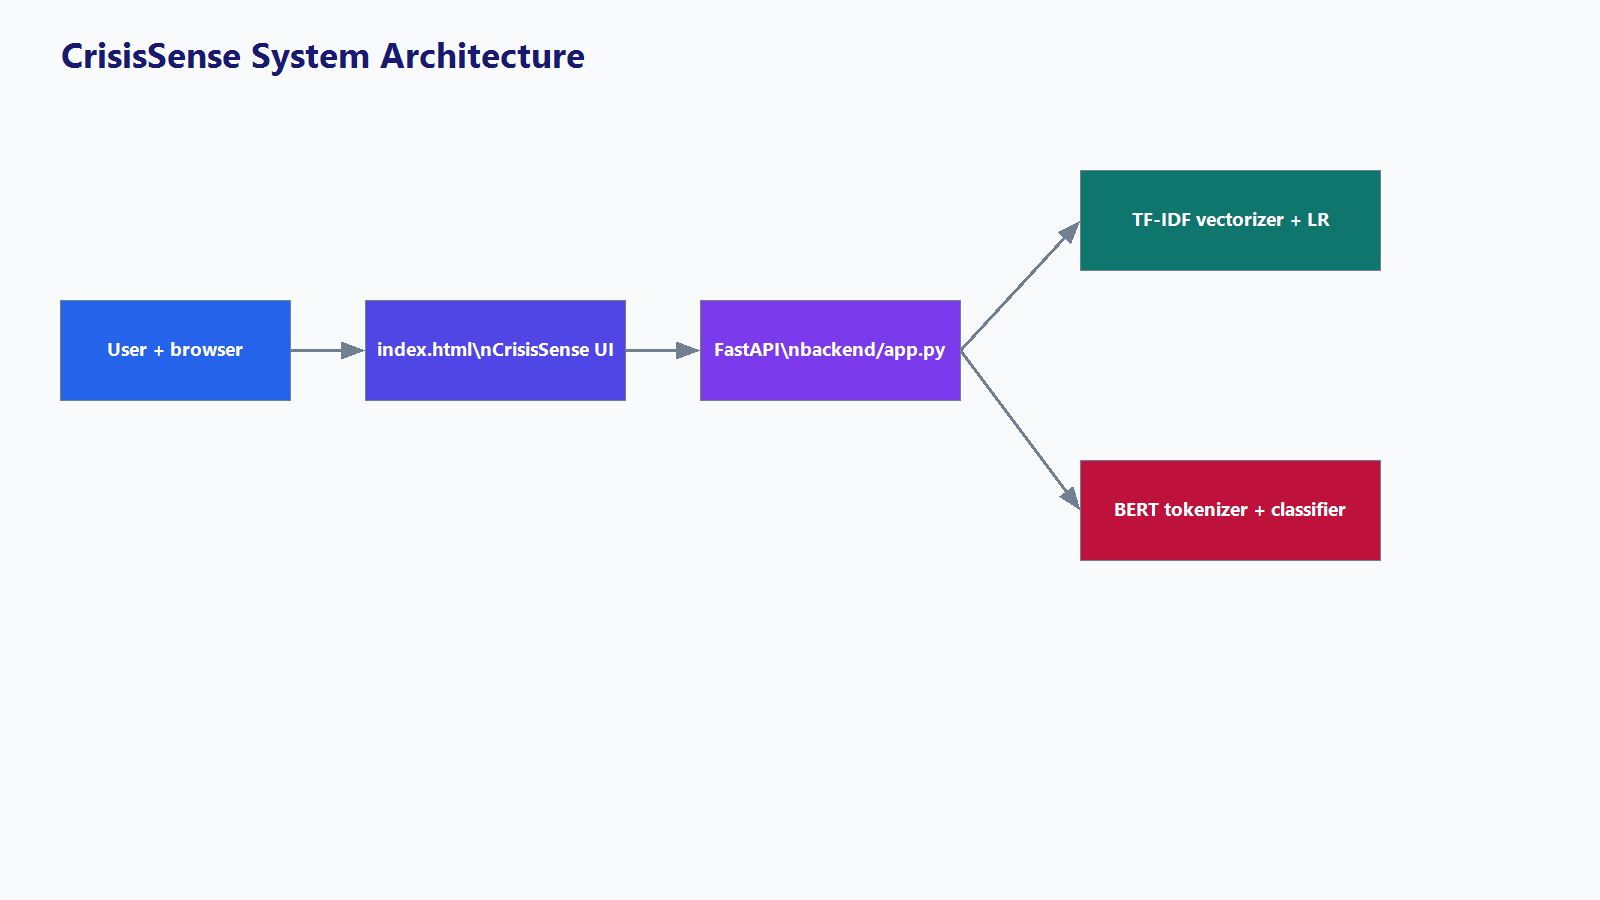
\includegraphics[width=0.85\textwidth]{system-architecture.png}
\caption{Overall CrisisSense system architecture. The frontend sends submitted text to \texttt{POST /\pbrk predict}; the FastAPI backend forwards it independently to the frozen TF-IDF/Logistic Regression pipeline and the frozen BERT pipeline, and returns both results to the frontend.}
\label{fig:system-architecture}
\end{figure}

\section{Frontend}

The frontend is a single static file, \texttt{index.html}, served directly by the FastAPI backend at \texttt{GET /\pbrk }. It loads Tailwind CSS from a CDN and requires no separate build step, local stylesheet, or JavaScript bundle. The interface has two views: a live-prediction view, which accepts free text and calls \texttt{POST /\pbrk predict}, displaying both models' predicted class, selected-class confidence, and whether the two models' numeric labels agree; and an "About CrisisSense" information view, which presents the class definitions, split counts, model comparison, confidence/agreement caveats, and three vetted evaluation figures served by the backend. Switching between the two views does not reload the page or trigger any retraining or refitting of the underlying models.

\section{FastAPI Backend}

The backend, \texttt{backend/\pbrk app.py}, is a single FastAPI application. It loads both frozen model artifacts once, at application startup, inside a \texttt{lifespan} context manager; if loading fails, the failure is recorded and \texttt{/\pbrk health} and \texttt{/\pbrk predict} respond with HTTP 503 rather than returning a fabricated prediction. This load-once pattern means that every request served during the application's lifetime uses the same in-memory model objects --- there is no per-request model loading and no per-request fitting.

\section{Frozen Model Artifacts}

Two artifact sets are loaded at startup:

\begin{itemize}[nosep]
  \item \textbf{TF-IDF + Logistic Regression}:\newline
  \texttt{models/tfidf\_\pbrk logistic\_\pbrk regression/tfidf\_\pbrk vectorizer.joblib} and\newline
  \texttt{models/tfidf\_\pbrk logistic\_\pbrk regression/logistic\_\pbrk regression.joblib}, both loaded with \texttt{joblib.load}.
  \item \textbf{BERT}: \texttt{models/\pbrk bert\_\pbrk no\_\pbrk severity/\pbrk }, loaded with Hugging Face's \texttt{AutoTokenizer} and \texttt{AutoModelForSequenceClassification}, using \texttt{local\_\pbrk files\_\pbrk only=True} so that no network call to a model hub occurs at runtime.
\end{itemize}

Figure~\ref{fig:artifact-lifecycle} traces these artifacts from the frozen dataset split, through the (separately recorded) training/freezing step for each model, to their two current uses: the offline evaluation script that produces the results in Chapter~\ref{ch:results}, and the live FastAPI inference path.

\begin{figure}[H]
\centering
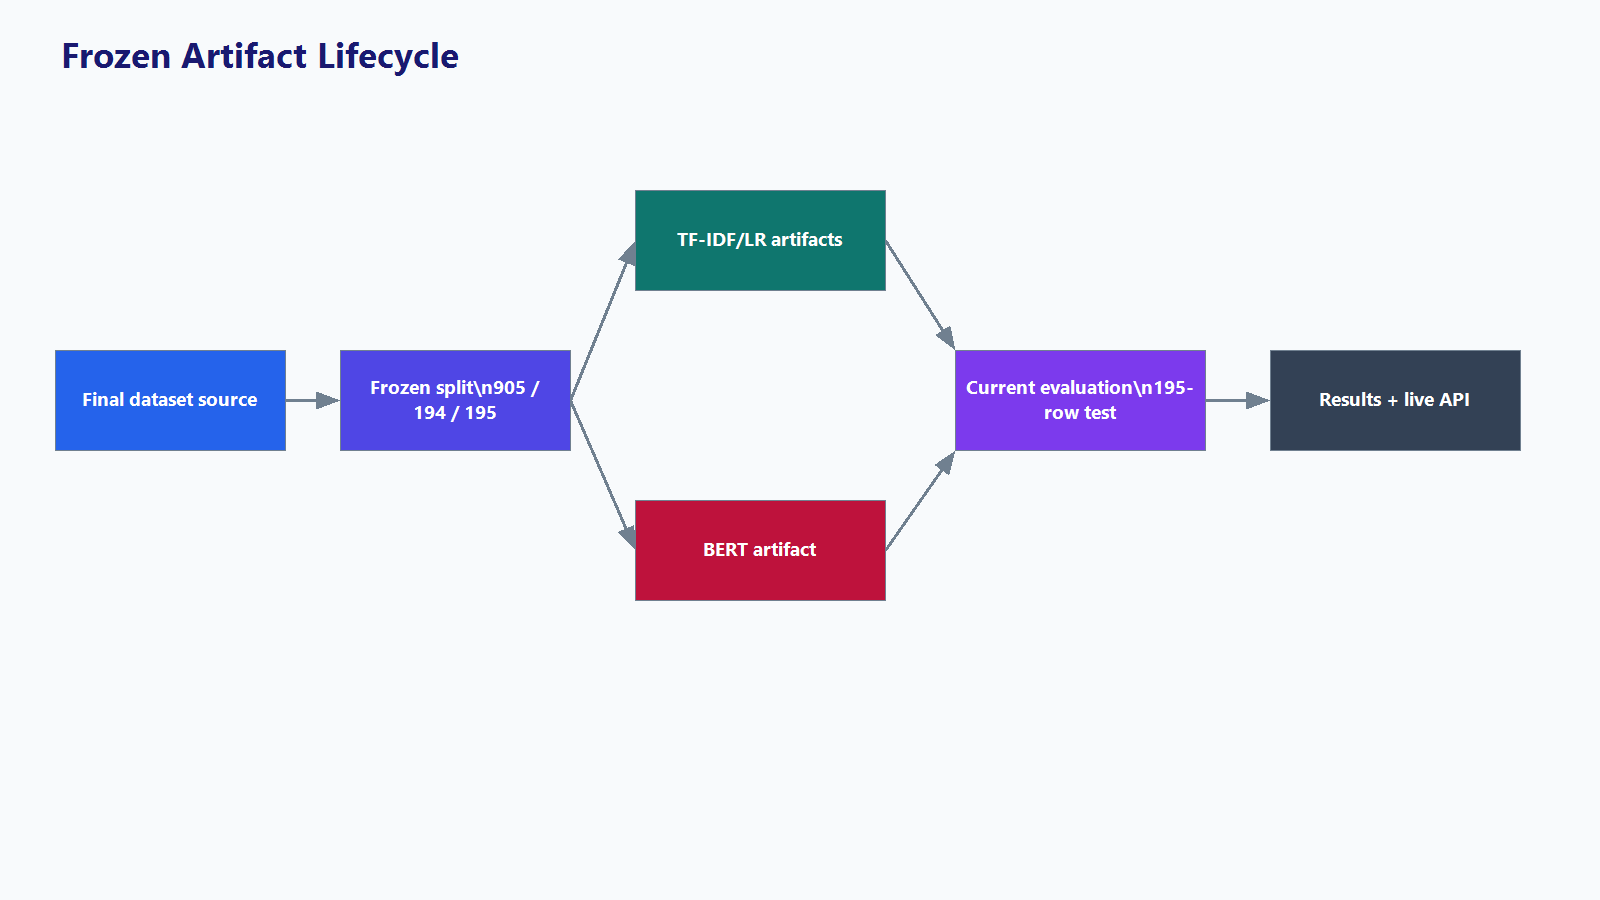
\includegraphics[width=0.85\textwidth]{artifact-lifecycle.png}
\caption{Frozen artifact lifecycle. The same TF-IDF/Logistic Regression and BERT artifacts feed both \texttt{scripts/\pbrk evaluate\_\pbrk current\_\pbrk models.py} (offline evaluation) and the live FastAPI \texttt{/\pbrk predict} endpoint (online inference); neither path fits, refits, or overwrites the artifacts.}
\label{fig:artifact-lifecycle}
\end{figure}

\section{Independent Model Paths}

The two models are structurally independent at every stage: separate representations (character-level TF-IDF vectors vs. BERT's contextual token representations), separate classifiers (Logistic Regression vs. a BERT sequence-classification head), and separate probability outputs. Figure~\ref{fig:model-comparison} shows the two paths side by side. Their outputs are never averaged, voted, stacked, or otherwise combined into a single ensemble prediction; the frontend and backend both treat them as two separate answers to the same question, and this report evaluates and discusses them as such throughout.

\begin{figure}[H]
\centering
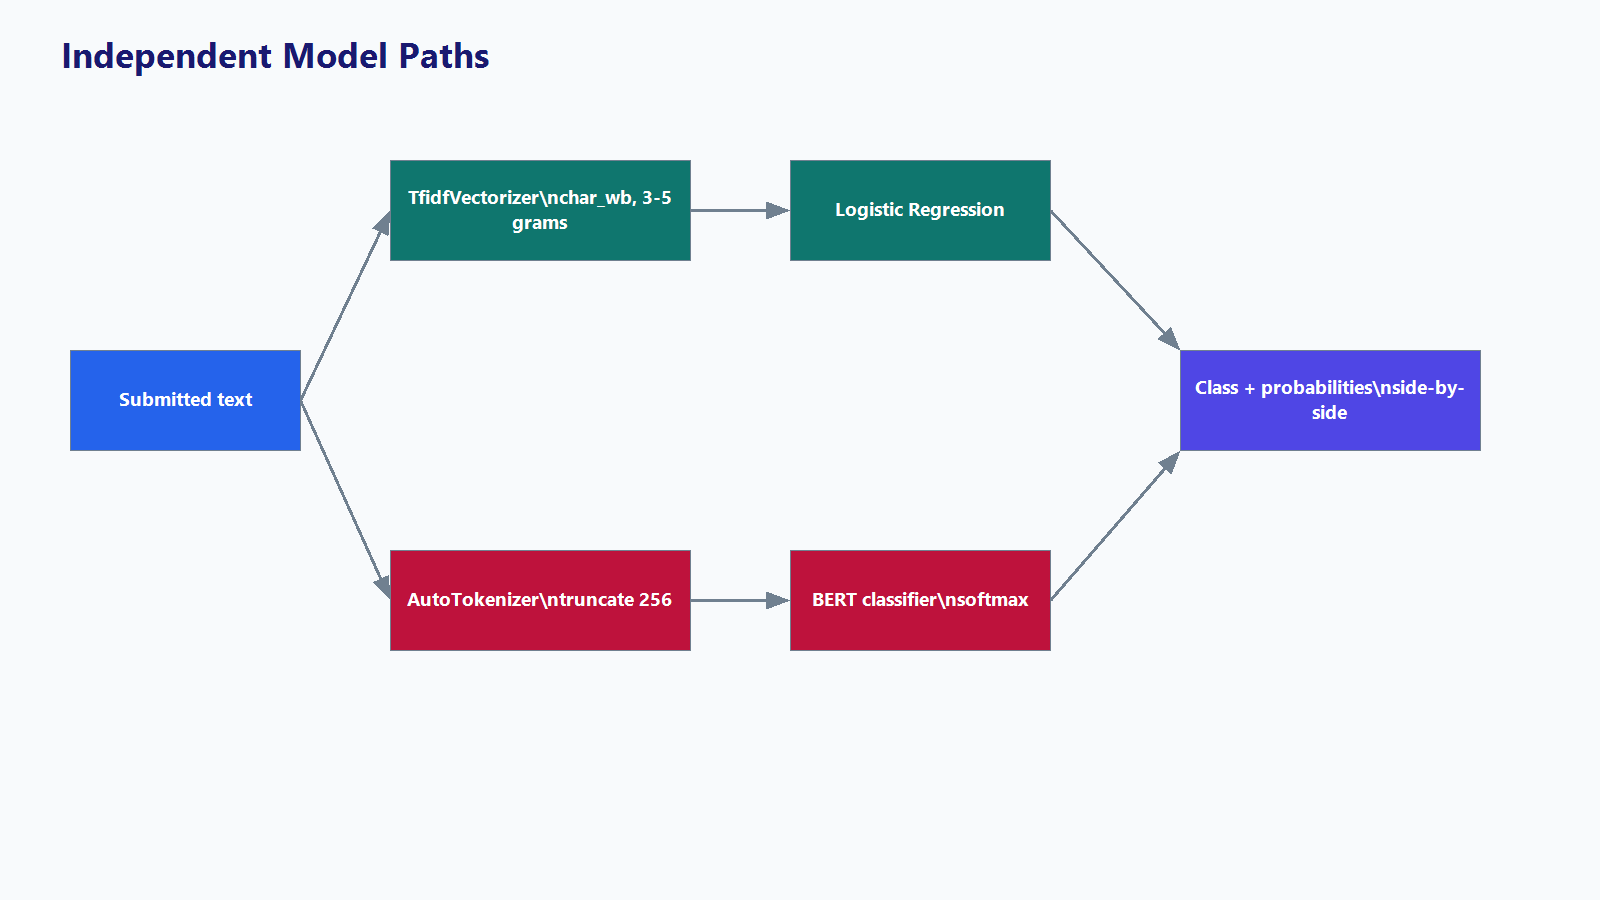
\includegraphics[width=0.85\textwidth]{model-comparison.png}
\caption{Independent model paths. Submitted text is processed separately by the TF-IDF + Logistic Regression pipeline and the BERT pipeline; each produces its own three-class probability distribution, and both are displayed together without being combined.}
\label{fig:model-comparison}
\end{figure}

\section{Prediction Flow}

Figure~\ref{fig:live-sequence} shows the sequence of calls triggered by a single live prediction request, from the user's text entry through both independent model paths to the JSON response returned to the frontend.

\begin{figure}[H]
\centering
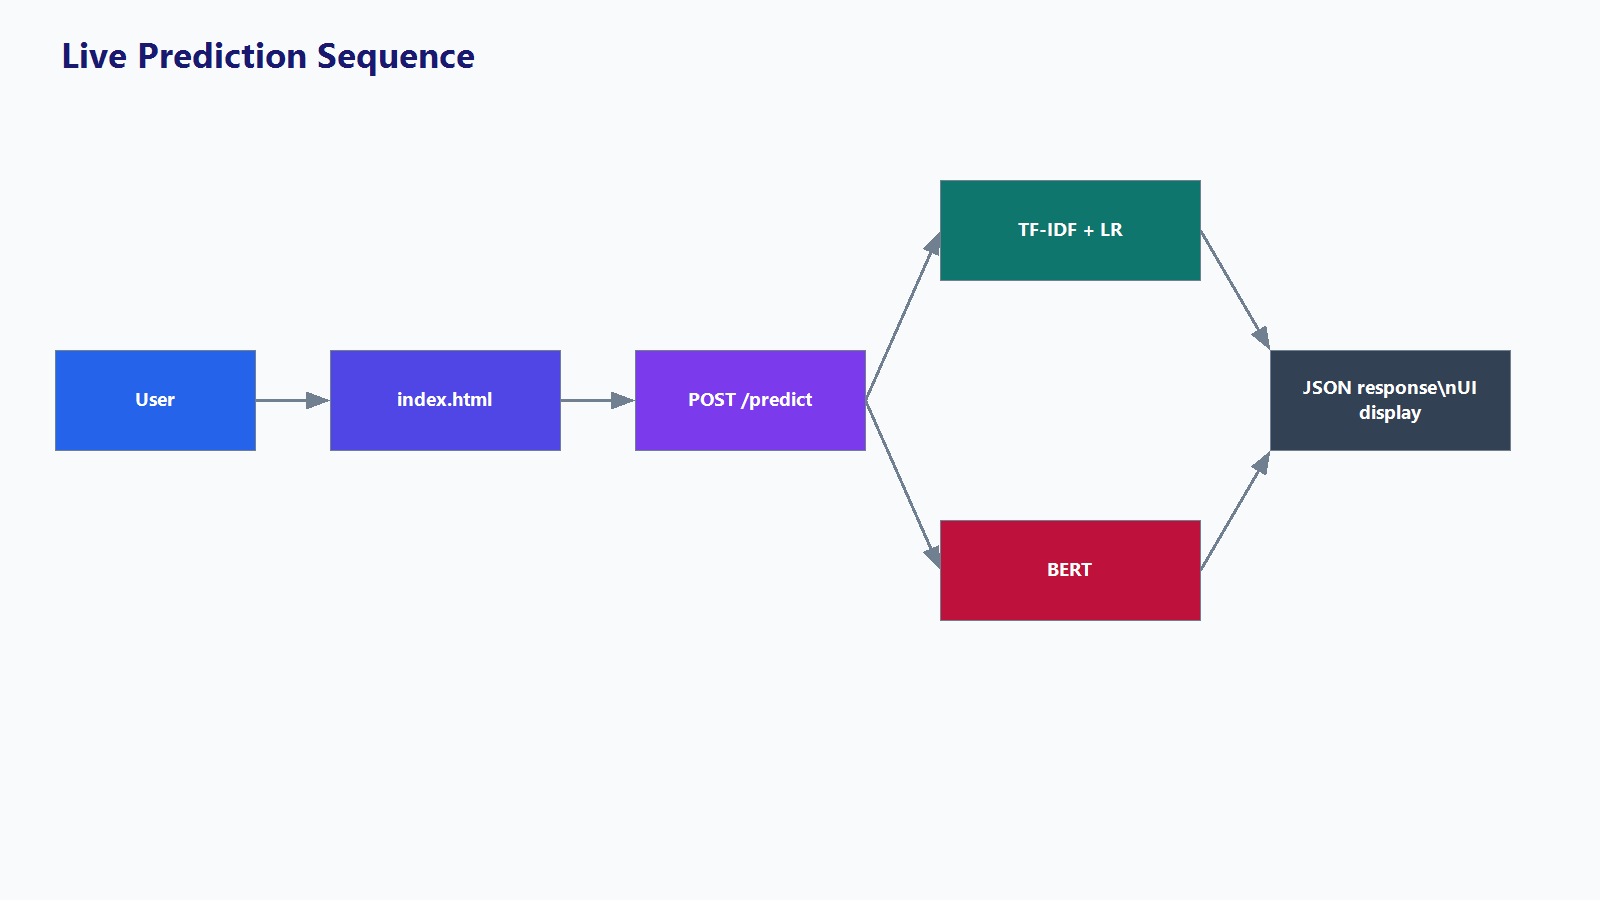
\includegraphics[width=0.85\textwidth]{live-prediction-sequence.png}
\caption{Live prediction sequence. A non-blank text submission is sent as JSON to \texttt{POST /\pbrk predict}; the backend runs the TF-IDF and BERT paths independently (conceptually in parallel) and returns both results together.}
\label{fig:live-sequence}
\end{figure}

\section{Runtime Architecture}

At runtime, TF-IDF inference runs entirely on CPU through scikit-learn sparse-matrix operations. BERT inference runs on CUDA if a GPU is available on the host machine, and falls back to CPU otherwise; when running on CPU, model weights are cast back to 32-bit floating point (\texttt{self.bert.float()}) to avoid precision issues associated with running half-precision weights without GPU support. Both models are placed in evaluation mode (\texttt{eval()}), and BERT inference additionally executes inside \texttt{torch.inference\_\pbrk mode()}, which disables gradient tracking and reduces memory overhead relative to ordinary forward-pass execution. No training, fitting, or artifact modification occurs anywhere in this runtime path.

\chapter{Methodology}
\label{ch:methodology}

\section{Overall Pipeline}

Both models consume the same raw \texttt{content} text and produce the same output shape: an integer label $\hat{y} \in \{0,1,2\}$ and a probability vector $(p_0, p_1, p_2)$ with $\sum_i p_i = 1$. They differ entirely in how text is represented and how the probability vector is computed. This chapter presents both pipelines in turn, followed by the metrics used to interpret confidence and agreement between the two.

\section{TF-IDF Representation}

Term Frequency--Inverse Document Frequency (TF-IDF) weights a term $t$ in a document $d$ by combining how often $t$ occurs in $d$ with how rare $t$ is across the whole corpus. Term frequency is

\begin{equation}
\mathrm{TF}(t,d) = \frac{\text{count of } t \text{ in } d}{\text{total terms in } d},
\end{equation}

and inverse document frequency, which down-weights terms that occur in most documents, is

\begin{equation}
\mathrm{IDF}(t) = \ln\!\left(\frac{N}{n_t}\right),
\end{equation}

where $N$ is the number of documents in the corpus and $n_t$ is the number of documents containing $t$. The combined weight is

\begin{equation}
\mathrm{TFIDF}(t,d) = \mathrm{TF}(t,d) \times \mathrm{IDF}(t).
\end{equation}

The frozen CrisisSense vectorizer additionally applies \emph{sublinear term-frequency scaling}, replacing raw term frequency with $1 + \ln(\mathrm{TF}(t,d))$ where $\mathrm{TF}(t,d) > 0$, which compresses the contribution of very frequently repeated terms within a single document.

\section{Character N-Grams}

Rather than treating whole words as terms, the frozen vectorizer uses the \texttt{char\_wb} analyzer, which extracts \emph{character n-grams within word boundaries}: contiguous sequences of 3 to 5 characters, taken from inside each whitespace-delimited word (padded at word edges), rather than sequences of whole words. This choice makes the representation robust to misspellings, informal punctuation, and morphological variation, since two differently spelled but visually similar tokens still share many overlapping character n-grams, whereas a word-level vectorizer would treat them as entirely unrelated vocabulary items. Table~\ref{tab:tfidf-config} gives the exact frozen configuration.

\begin{table}[H]
\centering
\caption{Frozen TF-IDF vectorizer configuration.}
\label{tab:tfidf-config}
\begin{tabular}{ll}
\toprule
\textbf{Setting} & \textbf{Value} \\
\midrule
Analyzer & \texttt{char\_wb} (character n-grams within word boundaries) \\
N-gram range & (3, 5) \\
\texttt{min\_df} & 2 \\
\texttt{max\_df} & 0.9 \\
\texttt{sublinear\_tf} & true \\
\texttt{max\_features} & 50{,}000 \\
Lowercase & true \\
Accent stripping & Unicode \\
Fitted features & 17{,}708 \\
Fitted on & training split only \\
\bottomrule
\end{tabular}
\end{table}

At inference time, the backend calls \texttt{vectorizer.transform([text])} directly on the raw submitted text. The verified live pipeline performs no separate stop-word removal, stemming, lemmatization, URL stripping, or manual punctuation removal beyond what the vectorizer itself performs (lowercasing and Unicode accent stripping); the \texttt{char\_wb} analyzer is responsible for deriving all downstream features.

\section{Logistic Regression}

The sparse TF-IDF feature vector is passed to a multinomial Logistic Regression classifier, which models the probability of each class $k$ given input features $x$ as a softmax over linear scores:

\begin{equation}
P(y = k \mid x) = \frac{\exp(w_k^\top x + b_k)}{\sum_{j=1}^{3} \exp(w_j^\top x + b_j)},
\end{equation}

where $w_k$ and $b_k$ are the learned weight vector and bias for class $k$. The frozen classifier configuration is given in Table~\ref{tab:lr-config}.

\begin{table}[H]
\centering
\caption{Frozen Logistic Regression configuration.}
\label{tab:lr-config}
\begin{tabular}{ll}
\toprule
\textbf{Setting} & \textbf{Value} \\
\midrule
$C$ (inverse regularization strength) & 1.0 \\
\texttt{class\_weight} & balanced \\
Solver & \texttt{lbfgs} \\
\texttt{max\_iter} & 5{,}000 \\
Random state & 42 \\
\bottomrule
\end{tabular}
\end{table}

The balanced class-weight setting reweights the training loss inversely proportional to class frequency, compensating for the moderate class imbalance shown in Table~\ref{tab:class-dist} (explicit-crisis is roughly 1.8$\times$ as frequent as implicit-crisis in the training split). At inference time, \texttt{predict\_proba} returns the full three-class probability vector and \texttt{predict} selects the arg-max label.

\section{BERT}

The BERT path replaces the sparse lexical representation entirely with a contextual transformer encoder. Given tokenized input $X = (x_1, \dots, x_n)$, each layer of the encoder computes scaled dot-product self-attention over the full sequence:

\begin{equation}
\mathrm{Attention}(Q, K, V) = \mathrm{softmax}\!\left(\frac{QK^\top}{\sqrt{d_k}}\right)V,
\end{equation}

where $Q$, $K$, and $V$ are learned linear projections of the layer's input and $d_k$ is the key dimension, allowing every token's representation to be updated using information drawn from every other token in the sequence rather than only from a fixed local window. Twelve such layers are stacked, each followed by a position-wise feed-forward network, producing a final contextual representation for every input token.

\section{Tokenization}

Raw text is tokenized locally with \texttt{AutoTokenizer} (\texttt{local\_\pbrk files\_\pbrk only=True}), which maps the input string to a sequence of subword token IDs plus an attention mask, using the vocabulary saved alongside the frozen model (\texttt{vocab\_size} = 30{,}522). Input is truncated to a maximum length of 256 tokens; text shorter than 256 tokens is not truncated, and no explicit padding strategy is set for a single-request inference call, since a batch of size one requires no padding.

\section{Transformer Encoder}

The saved BERT configuration (Table~\ref{tab:bert-config}) specifies a standard \texttt{BertForSequenceClassification} architecture: 12 transformer encoder layers, a hidden size of 768, and 12 attention heads per layer. The final contextual representation of the special classification token is taken as a fixed-size pooled representation of the entire input sequence.

\begin{table}[H]
\centering
\caption{Frozen BERT architecture configuration (from \texttt{models/\pbrk bert\_\pbrk no\_\pbrk severity/\pbrk config.json}).}
\label{tab:bert-config}
\begin{tabular}{ll}
\toprule
\textbf{Setting} & \textbf{Value} \\
\midrule
Architecture & \texttt{BertForSequenceClassification} \\
Hidden layers & 12 \\
Hidden size & 768 \\
Attention heads & 12 \\
Vocabulary size & 30{,}522 \\
Max position embeddings & 512 \\
Output labels & 3 \\
Max input length used at inference & 256 tokens \\
\bottomrule
\end{tabular}
\end{table}

\section{Classification Head}

A linear classification head maps the pooled 768-dimensional representation to three raw scores (logits), one per class, mirroring the linear-then-softmax structure of the Logistic Regression path but operating on a learned contextual representation rather than a sparse lexical one.

\section{Softmax Probabilities}

The three logits $z = (z_0, z_1, z_2)$ are converted into a probability distribution with the standard softmax function,

\begin{equation}
P(y = k \mid x) = \frac{\exp(z_k)}{\sum_{j=1}^{3} \exp(z_j)},
\end{equation}

and the predicted class is $\hat{y} = \arg\max_k P(y=k \mid x)$. This computation is performed under \texttt{torch.inference\_\pbrk mode()}, which disables autograd bookkeeping since no training occurs at this stage.

\begin{quote}
\raggedright\small
\begin{verbatim}
Raw text -> local BERT tokenizer (truncate to 256)
         -> token IDs + attention mask
         -> BERT transformer encoder (12 layers)
         -> pooled contextual representation
         -> linear classification head -> logits
         -> softmax -> three class probabilities
         -> predicted class
\end{verbatim}
\end{quote}

\section{Confidence}

For both models, \emph{confidence} is defined as the probability mass assigned to the predicted (selected) class, $p_{\hat{y}} = \max_k P(y=k \mid x)$. Confidence is a property of the model's own output distribution, not a measurement of correctness; a model can be simultaneously highly confident and wrong, or cautious and correct. Chapter~\ref{ch:results} reports confidence statistics and calibration error precisely because these two models exhibit very different confidence behavior that is not explained by their accuracy difference alone.

\section{Model Agreement}

Because TF-IDF/Logistic Regression and BERT are evaluated independently on the same input, it is possible to ask, for each test example, whether their predicted labels $\hat{y}_{\mathrm{tfidf}}$ and $\hat{y}_{\mathrm{bert}}$ coincide. \emph{Agreement} is defined simply as $\hat{y}_{\mathrm{tfidf}} = \hat{y}_{\mathrm{bert}}$, without reference to the true label; it is a measure of consistency between two independent classifiers, not a measure of correctness, and Chapter~\ref{ch:results} reports agreement and per-model correctness as separate quantities.

\chapter{Implementation}

\section{Software Stack}

CrisisSense's current runtime stack is summarized in Table~\ref{tab:software-stack}.

\begin{table}[H]
\centering
\caption{Current software and environment stack.}
\label{tab:software-stack}
\begin{tabular}{ll}
\toprule
\textbf{Component} & \textbf{Library / Requirement} \\
\midrule
Language & Python 3.10+ \\
Web framework & FastAPI ($\geq$0.116), Uvicorn ($\geq$0.35) \\
Classical ML & scikit-learn ($\geq$1.3), joblib ($\geq$1.3) \\
Data handling & pandas ($\geq$2.0), NumPy ($\geq$1.24) \\
Deep learning & PyTorch ($\geq$2.0), Transformers ($\geq$4.35), Accelerate ($\geq$0.24) \\
Frontend & Static HTML (\texttt{index.html}) with Tailwind CSS via CDN \\
Artifact versioning & Git LFS (tracks \texttt{.joblib} and BERT weight files) \\
\bottomrule
\end{tabular}
\end{table}

Core dependencies are declared in \texttt{requirements.txt}; the BERT-specific dependencies (PyTorch~\cite{paszke2019pytorch}, Transformers~\cite{wolf2020transformers}, Accelerate) are declared separately in \texttt{requirements-ml.txt}, which installs on top of the core requirements. The TF-IDF and Logistic Regression artifacts are produced with scikit-learn~\cite{pedregosa2011scikit}.

\section{Repository Structure}

Table~\ref{tab:repo-structure} lists the repository paths that constitute the current deployed system, as distinguished from historical research material retained elsewhere in the repository (Section~\ref{sec:runtime-boundary}).

\begin{table}[H]
\centering
\small
\caption{Current-system file map.}
\label{tab:repo-structure}
\begin{tabular}{p{4.3cm}p{8.7cm}}
\toprule
\textbf{Path} & \textbf{Purpose} \\
\midrule
\texttt{index.html} & CrisisSense frontend. \\
\texttt{backend/\pbrk app.py} & FastAPI application: model loading, endpoints, prediction. \\
\texttt{data/\pbrk final\_\pbrk datasets/\pbrk splits/\pbrk } & Frozen train/validation/test CSV copies. \\
\texttt{models/\pbrk tfidf\_\pbrk logistic\_\pbrk regression/\pbrk } & Frozen TF-IDF vectorizer and Logistic Regression artifacts. \\
\texttt{models/\pbrk bert\_\pbrk no\_\pbrk severity/\pbrk } & Frozen BERT weights, tokenizer, and configuration. \\
\texttt{configs/\pbrk tfidf\_\pbrk final\_\pbrk frozen.json} & Freeze record declaring the final TF-IDF/LR settings. \\
\texttt{scripts/\pbrk evaluate\_\pbrk current\_\pbrk models.py} & Offline evaluation of both frozen models on \texttt{test.csv}. \\
\texttt{results/\pbrk model\_\pbrk comparison/\pbrk } & Current metrics, prediction table, summary, and figures. \\
\texttt{tests/\pbrk test\_\pbrk inference\_\pbrk api.py} & Smoke tests for \texttt{/\pbrk health} and \texttt{/\pbrk predict}. \\
\texttt{New\_docs/\pbrk } & Current-project documentation and architecture diagrams. \\
\bottomrule
\end{tabular}
\end{table}

\section{Model Artifacts}

The TF-IDF and Logistic Regression artifacts are serialized with \texttt{joblib} as two separate \texttt{.joblib} files, loaded with \texttt{joblib.load} at application startup. The BERT artifact is stored as a standard Hugging Face model directory (\texttt{model.safetensors}, \texttt{config.json}, \texttt{tokenizer.json}, \texttt{tokenizer\_\pbrk config.json}) and loaded with \texttt{AutoTokenizer.from\_\pbrk pretrained} and \texttt{AutoModelForSequenceClassification.from\_\pbrk pretrained}, both called with \texttt{local\_\pbrk files\_\pbrk only=True} to guarantee that no network request to a remote model hub occurs during application startup or at inference time. All of these artifact files are tracked with Git LFS, as declared in \texttt{.gitattributes}.

\section{Backend Implementation}

The backend centers on a single \texttt{FrozenModels} class, instantiated once inside the FastAPI \texttt{lifespan} context manager and stored on \texttt{app.state.models}. It exposes two prediction methods, \texttt{predict\_tfidf} and \texttt{predict\_bert}, each of which is a pure inference call against the already-loaded artifacts: neither method fits, refits, retrains, or writes to any model artifact. If artifact loading fails at startup, \texttt{app.state.models} is set to \texttt{None} and the error message is recorded on \texttt{app.state.load\_\pbrk error}; \texttt{/\pbrk health} and \texttt{/\pbrk predict} then respond with HTTP 503 rather than silently returning an incorrect or placeholder prediction.

\section{API Endpoints}

Table~\ref{tab:api-endpoints} documents the backend's five endpoints.

\begin{table}[H]
\centering
\caption{Current backend API endpoints.}
\label{tab:api-endpoints}
\begin{tabular}{lp{9.5cm}}
\toprule
\textbf{Endpoint} & \textbf{Purpose} \\
\midrule
\texttt{GET /\pbrk } & Serves \texttt{index.html}. \\
\texttt{GET /\pbrk health} & Reports model load status; HTTP 503 if artifacts failed to load. \\
\texttt{GET /\pbrk project-info} & Reads current split row counts; returns totals, input/target field names, and class count. \\
\texttt{GET /\pbrk evaluation/\pbrk \{filename\}} & Serves only the three frontend-approved evaluation graphs (overall metrics, per-class F1, confidence distribution); any other filename returns HTTP 404. \\
\texttt{POST /\pbrk predict} & Accepts \texttt{\{"text": "..."\}}; returns independent TF-IDF and BERT predictions. Blank text is rejected with HTTP 422. \\
\bottomrule
\end{tabular}
\end{table}

Each model object in a \texttt{/\pbrk predict} response contains a \texttt{label} (integer), a \texttt{class\_name} (string), and a \texttt{probabilities} object keyed by the three class names, so that the frontend can render both the predicted class and the full probability distribution for each model.

\section{Frontend}

As described in Section~\ref{ch:architecture}, the frontend is a single static HTML page with no separate build pipeline. It performs two kinds of network calls: \texttt{POST /\pbrk predict} for live classification requests, and \texttt{GET /\pbrk project-info} plus \texttt{GET /\pbrk evaluation/\pbrk \{filename\}} for populating the information view with dataset counts and the three vetted evaluation figures.

\section{Runtime Inference}

A single \texttt{POST /\pbrk predict} request triggers, in sequence within the request handler: a Pydantic validation check that the submitted text is non-blank; a call to \texttt{FrozenModels.predict\_\pbrk tfidf}, which transforms the text with the frozen vectorizer and calls \texttt{predict\_proba} and \texttt{predict} on the frozen Logistic Regression classifier; and a call to \texttt{FrozenModels.predict\_\pbrk bert}, which tokenizes the text, truncates to 256 tokens, runs a forward pass under \texttt{torch.inference\_\pbrk mode()}, and applies softmax to the resulting logits. Both results are assembled into a single JSON response and returned to the frontend. No step in this path performs gradient computation, parameter updates, or artifact writes.

\section{Reproducibility}
\label{sec:reproducibility}

The documented current launch sequence is:

\begin{lstlisting}[language=bash]
python -m venv .venv
.\.venv\Scripts\Activate.ps1
pip install -r requirements-ml.txt
git lfs pull
python -m uvicorn backend.app:app --host 127.0.0.1 --port 8000
\end{lstlisting}

After these steps, the application is available at \texttt{http:/\pbrk /\pbrk 127.0.0.1:8000/\pbrk }; the FastAPI process serves both the API and the static frontend, so no separate frontend build or server is required. \texttt{git lfs pull} must be run after cloning, before starting the API, because the vectorizer, classifier, and BERT weight files are stored through Git LFS rather than committed as ordinary blobs. This report's reproducibility claim is scoped to \emph{inference} using the already-frozen artifacts and to \emph{offline evaluation} via \texttt{scripts/\pbrk evaluate\_\pbrk current\_\pbrk models.py}; it does not claim that the BERT artifact's original fine-tuning process is reproduced from this repository state, since that training script belongs to a separate, historical part of the repository (Section~\ref{sec:runtime-boundary}).

\label{sec:runtime-boundary}
\paragraph{Current-system boundary.} The repository additionally retains earlier four-class gold-data, annotation, notebook, and BERT training modules under paths such as \texttt{src/\pbrk models/\pbrk bert/\pbrk }, \texttt{scripts/\pbrk models/\pbrk }, and \texttt{annotation/\pbrk }. These use different label schemes (including a \texttt{hard\_negative} label), different split sizes, and different artifact paths, and are historical research material. They are not used by the current frontend, backend, frozen split, or frozen models, and are excluded from this report's technical content and results.

\chapter{Experimental Setup}
\label{ch:experimental-setup}

\section{Test Protocol}

Both frozen models are evaluated by \texttt{scripts/\pbrk evaluate\_\pbrk current\_\pbrk models.py}, which loads the same \texttt{FrozenModels} class used by the live FastAPI backend and applies its \texttt{predict\_tfidf} and \texttt{predict\_bert} methods to every row of \texttt{data/\pbrk final\_\pbrk datasets/\pbrk splits/\pbrk test.csv} (195 rows). Using the identical inference path as the deployed API ensures that the reported evaluation numbers describe the system as it is actually served, rather than a separately reimplemented evaluation pipeline that could silently diverge from production behavior. The script writes its outputs to \texttt{results/\pbrk model\_\pbrk comparison/\pbrk }: \texttt{metrics.csv}, \texttt{metrics.json}, \texttt{per\_\pbrk class\_\pbrk metrics.csv}, \texttt{predictions.csv} (per-row ground truth, both predictions, both confidences, correctness flags, and an agreement flag), \texttt{evaluation\_\pbrk summary.md}, and the figures discussed in Chapter~\ref{ch:results}. Figure~\ref{fig:dataset-evaluation} summarizes this evaluation flow end to end.

\begin{figure}[H]
\centering
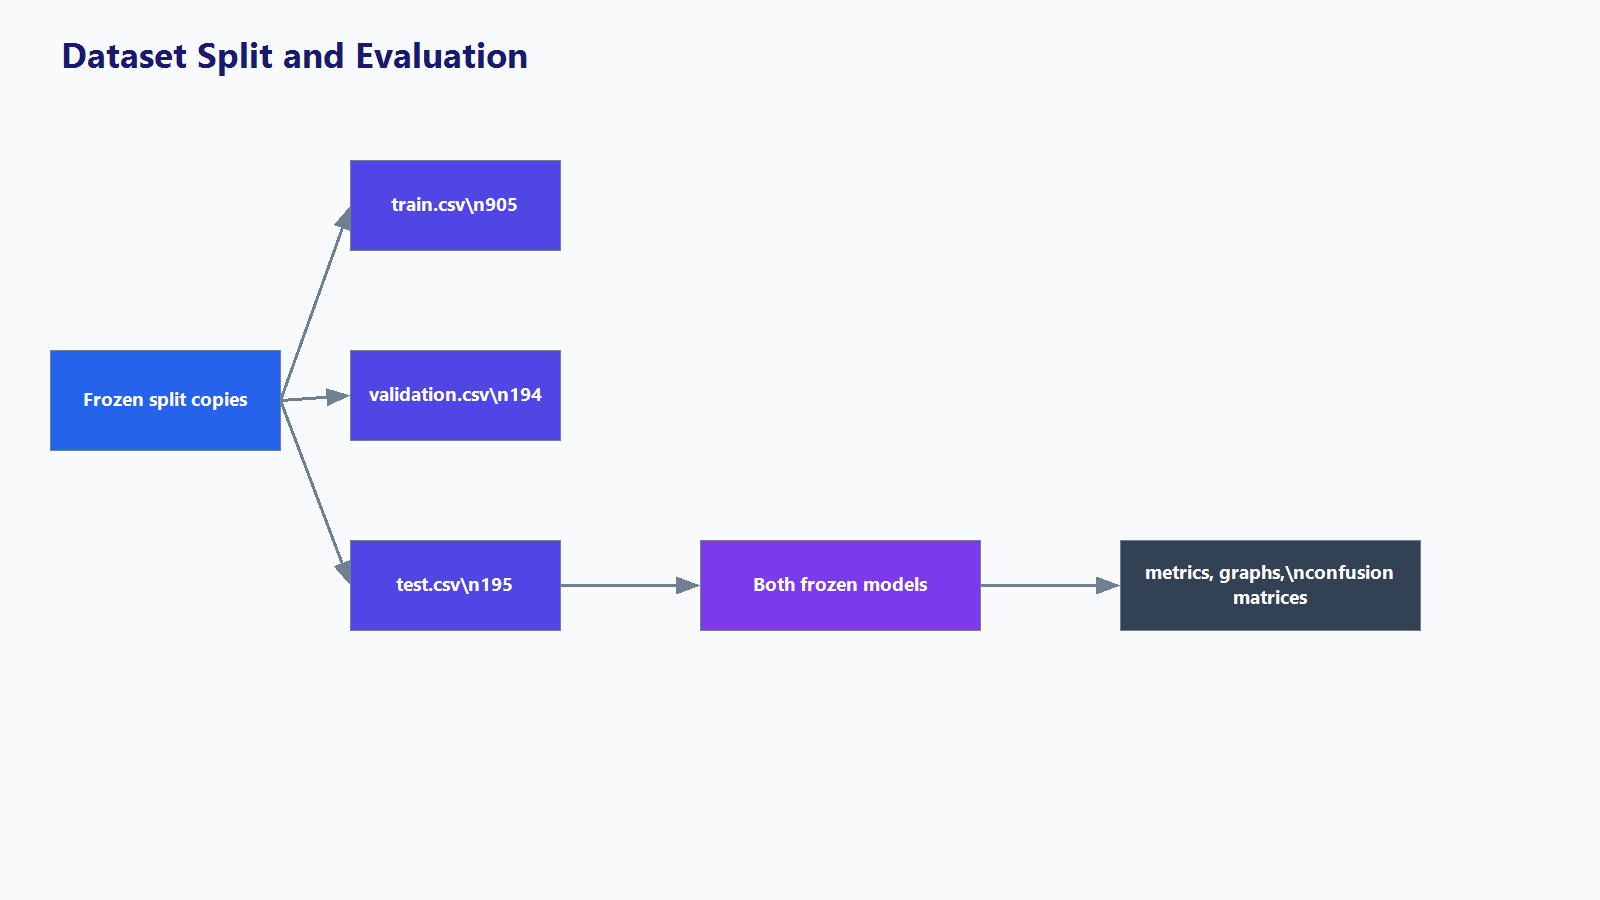
\includegraphics[width=0.85\textwidth]{dataset-evaluation.png}
\caption{Dataset-to-evaluation flow. The frozen split feeds both frozen models identically; predictions on the shared 195-row test set are aggregated into metrics, confusion matrices, and the presentation figures used throughout Chapter~\ref{ch:results}.}
\label{fig:dataset-evaluation}
\end{figure}

\section{Evaluation Metrics}

The metrics below are computed once per model over all 195 test rows and, where noted, per class.

\subsection{Accuracy}

\begin{equation}
\mathrm{Accuracy} = \frac{\text{number of correct predictions}}{\text{total predictions}}.
\end{equation}

\subsection{Precision}

For a given class $k$, with $TP_k$, $FP_k$ true/false positives for that class,

\begin{equation}
\mathrm{Precision}_k = \frac{TP_k}{TP_k + FP_k}.
\end{equation}

\subsection{Recall}

\begin{equation}
\mathrm{Recall}_k = \frac{TP_k}{TP_k + FN_k}.
\end{equation}

\subsection{F1 Score}

\begin{equation}
F1_k = \frac{2 \cdot \mathrm{Precision}_k \cdot \mathrm{Recall}_k}{\mathrm{Precision}_k + \mathrm{Recall}_k}.
\end{equation}

\subsection{Macro-F1}

Macro-averaging computes each metric independently per class and takes the unweighted mean across classes, so that the smaller implicit-crisis class contributes equally to the aggregate score despite having fewer test examples than explicit-crisis:

\begin{equation}
\mathrm{Macro\text{-}F1} = \frac{F1_{\text{no\_crisis}} + F1_{\text{implicit\_crisis}} + F1_{\text{explicit\_crisis}}}{3}.
\end{equation}

Macro-averaged precision and recall are computed analogously.

\subsection{Confusion Matrix}

A $3\times3$ confusion matrix $C$ is computed per model, where $C_{i,j}$ is the number of test examples with true label $i$ predicted as label $j$, ordered no-crisis, implicit-crisis, explicit-crisis. Diagonal entries are correct predictions; off-diagonal entries are misclassifications, and their pattern reveals \emph{which} classes a model confuses, information that overall accuracy alone does not provide.

\subsection{Confidence}

As defined in Section~\ref{ch:methodology}, confidence for a given prediction is $p_{\hat{y}} = \max_k P(y=k\mid x)$, the probability mass on the selected class. Mean and median confidence are reported per model over all 195 test predictions.

\subsection{Expected Calibration Error}

Expected Calibration Error (ECE) measures how far a model's confidence tracks its actual accuracy. Predictions are partitioned into $B$ confidence bins; within each bin $b$, the observed accuracy $\mathrm{acc}(b)$ is compared to the mean predicted confidence $\mathrm{conf}(b)$, and the discrepancies are averaged, weighted by bin size:

\begin{equation}
\mathrm{ECE} = \sum_{b=1}^{B} \frac{n_b}{N} \left| \mathrm{acc}(b) - \mathrm{conf}(b) \right|,
\end{equation}

where $n_b$ is the number of predictions in bin $b$ and $N = 195$ is the total number of test predictions. A perfectly calibrated model has $\mathrm{ECE} = 0$; a model that is systematically overconfident produces $\mathrm{conf}(b) > \mathrm{acc}(b)$ in most bins.

\subsection{Model Agreement}

Agreement is the fraction of test examples on which $\hat{y}_{\mathrm{tfidf}} = \hat{y}_{\mathrm{bert}}$, reported both in aggregate and (Chapter~\ref{ch:results}) broken down by predicted class.

\section{Summary of Setup}

Table~\ref{tab:eval-setup} summarizes the fixed evaluation configuration used to produce every result in Chapter~\ref{ch:results}.

\begin{table}[H]
\centering
\caption{Evaluation configuration summary.}
\label{tab:eval-setup}
\begin{tabular}{lp{9.5cm}}
\toprule
\textbf{Setting} & \textbf{Value} \\
\midrule
Evaluation script & \texttt{scripts/evaluate\_current\_models.py} \\
Inference path & Identical to \texttt{backend.app.FrozenModels} (live API path) \\
Test set & \texttt{data/final\_datasets/splits/test.csv}, 195 rows \\
No.\ of classes & 3 \\
Input field / target field & \texttt{content} / \texttt{label} \\
Calibration bins & 10 \\
Output artifacts & metrics.csv, metrics.json, per\_class\_metrics.csv, predictions.csv, figures \\
\bottomrule
\end{tabular}
\end{table}

\chapter{Results}
\label{ch:results}

\section{Overall Model Comparison}

Table~\ref{tab:overall-metrics} gives the overall test-set metrics for both models, and Figure~\ref{fig:overall-metrics} presents the same comparison graphically.

\begin{table}[H]
\centering
\caption{Overall test-set metrics (195 test rows).}
\label{tab:overall-metrics}
\begin{tabular}{lrr}
\toprule
\textbf{Metric} & \textbf{TF-IDF + LR} & \textbf{BERT} \\
\midrule
Accuracy         & 71.28\% & 76.92\% \\
Macro Precision  & 70.07\% & 75.10\% \\
Macro Recall     & 69.79\% & 74.44\% \\
Macro F1         & 69.62\% & 74.66\% \\
\bottomrule
\end{tabular}
\end{table}

\begin{figure}[H]
\centering
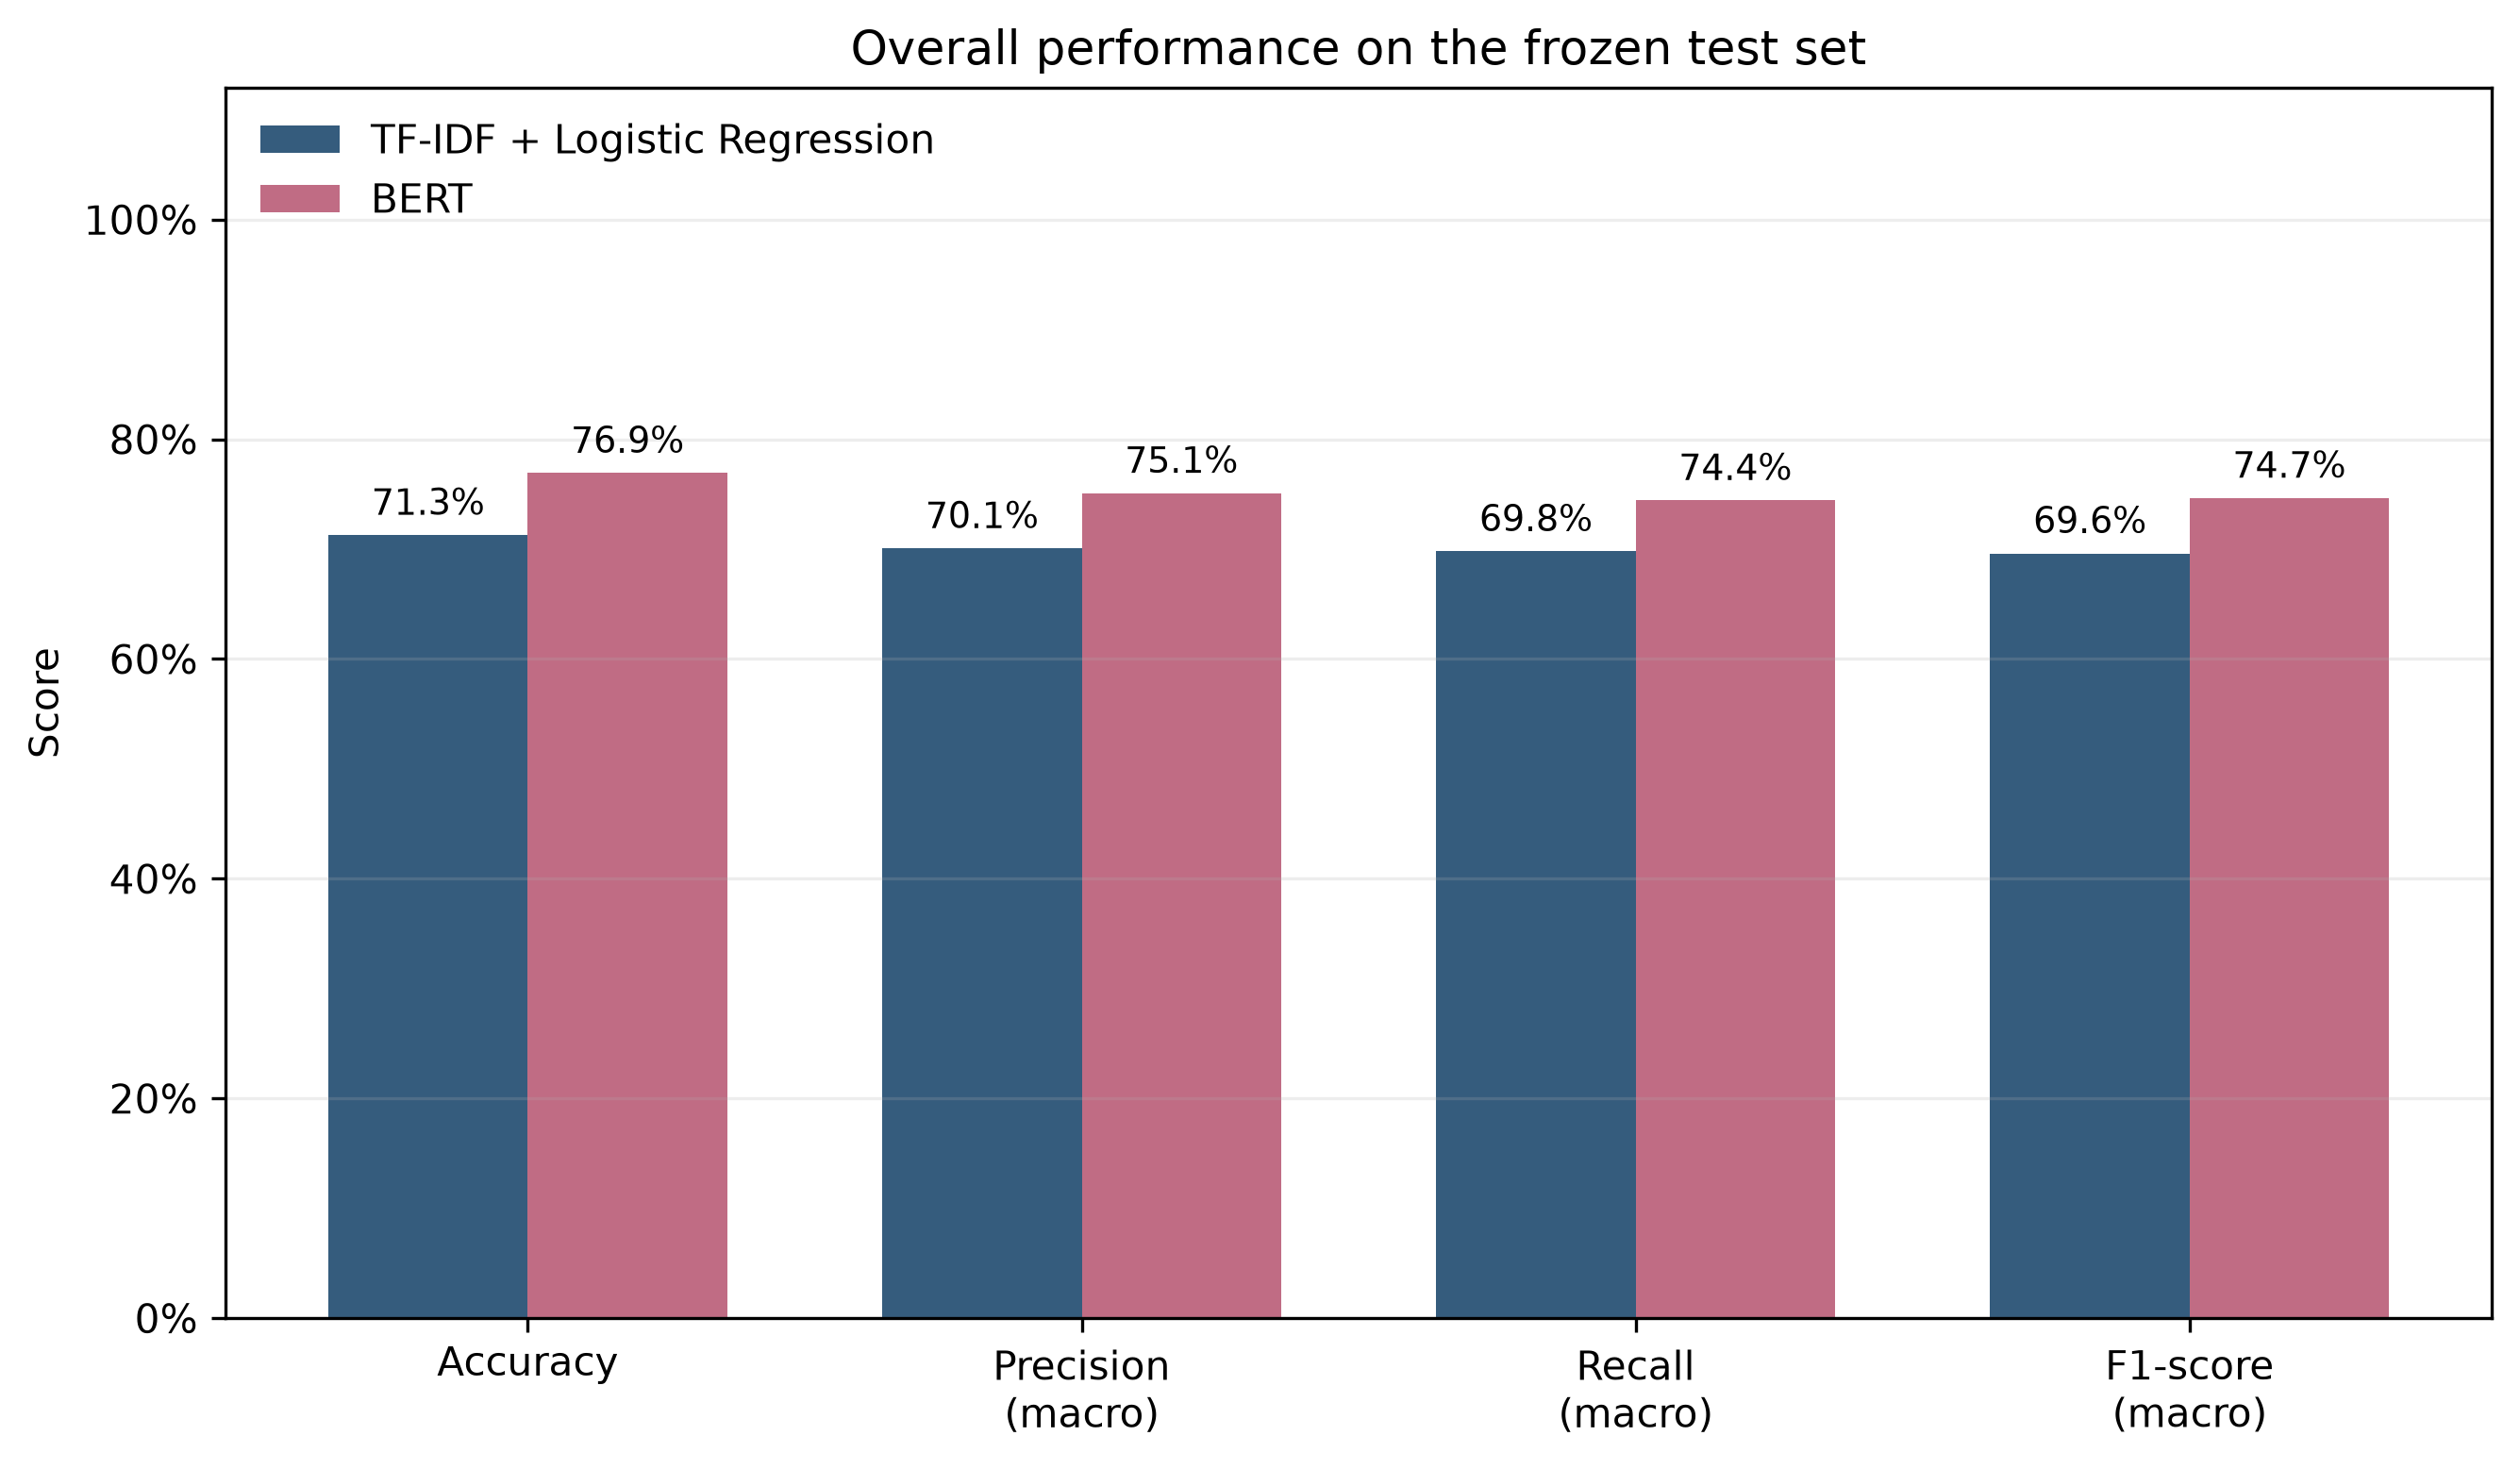
\includegraphics[width=0.8\textwidth]{overall_metrics.png}
\caption{Overall accuracy, macro precision, macro recall, and macro F1 for TF-IDF + Logistic Regression versus BERT on the shared 195-row test set.}
\label{fig:overall-metrics}
\end{figure}

BERT achieves higher accuracy and macro F1 than TF-IDF + Logistic Regression on every overall metric in Table~\ref{tab:overall-metrics}, by a margin of roughly 5--6 percentage points. This aggregate advantage, however, does not automatically extend to every individual class, as Section~\ref{sec:per-class-results} shows.

\section{Per-Class Results}
\label{sec:per-class-results}

Table~\ref{tab:per-class} gives precision, recall, F1, and support for each class and model, drawn directly from \texttt{results/\pbrk model\_\pbrk comparison/\pbrk per\_\pbrk class\_\pbrk metrics.csv}. Figure~\ref{fig:per-class-f1} plots the F1 comparison.

\begin{table}[H]
\centering
\caption{Per-class precision, recall, F1, and support on the 195-row test set.}
\label{tab:per-class}
\begin{tabular}{llrrrr}
\toprule
\textbf{Model} & \textbf{Class} & \textbf{Precision} & \textbf{Recall} & \textbf{F1} & \textbf{Support} \\
\midrule
TF-IDF + LR & No Crisis       & 70.45\% & 58.49\% & 63.92\% & 53 \\
TF-IDF + LR & Implicit Crisis & 63.16\% & 73.47\% & 67.92\% & 49 \\
TF-IDF + LR & Explicit Crisis & 76.60\% & 77.42\% & 77.01\% & 93 \\
\midrule
BERT & No Crisis       & 76.60\% & 67.92\% & 72.00\% & 53 \\
BERT & Implicit Crisis & 65.38\% & 69.39\% & 67.33\% & 49 \\
BERT & Explicit Crisis & 83.33\% & 86.02\% & 84.66\% & 93 \\
\bottomrule
\end{tabular}
\end{table}

\begin{figure}[H]
\centering
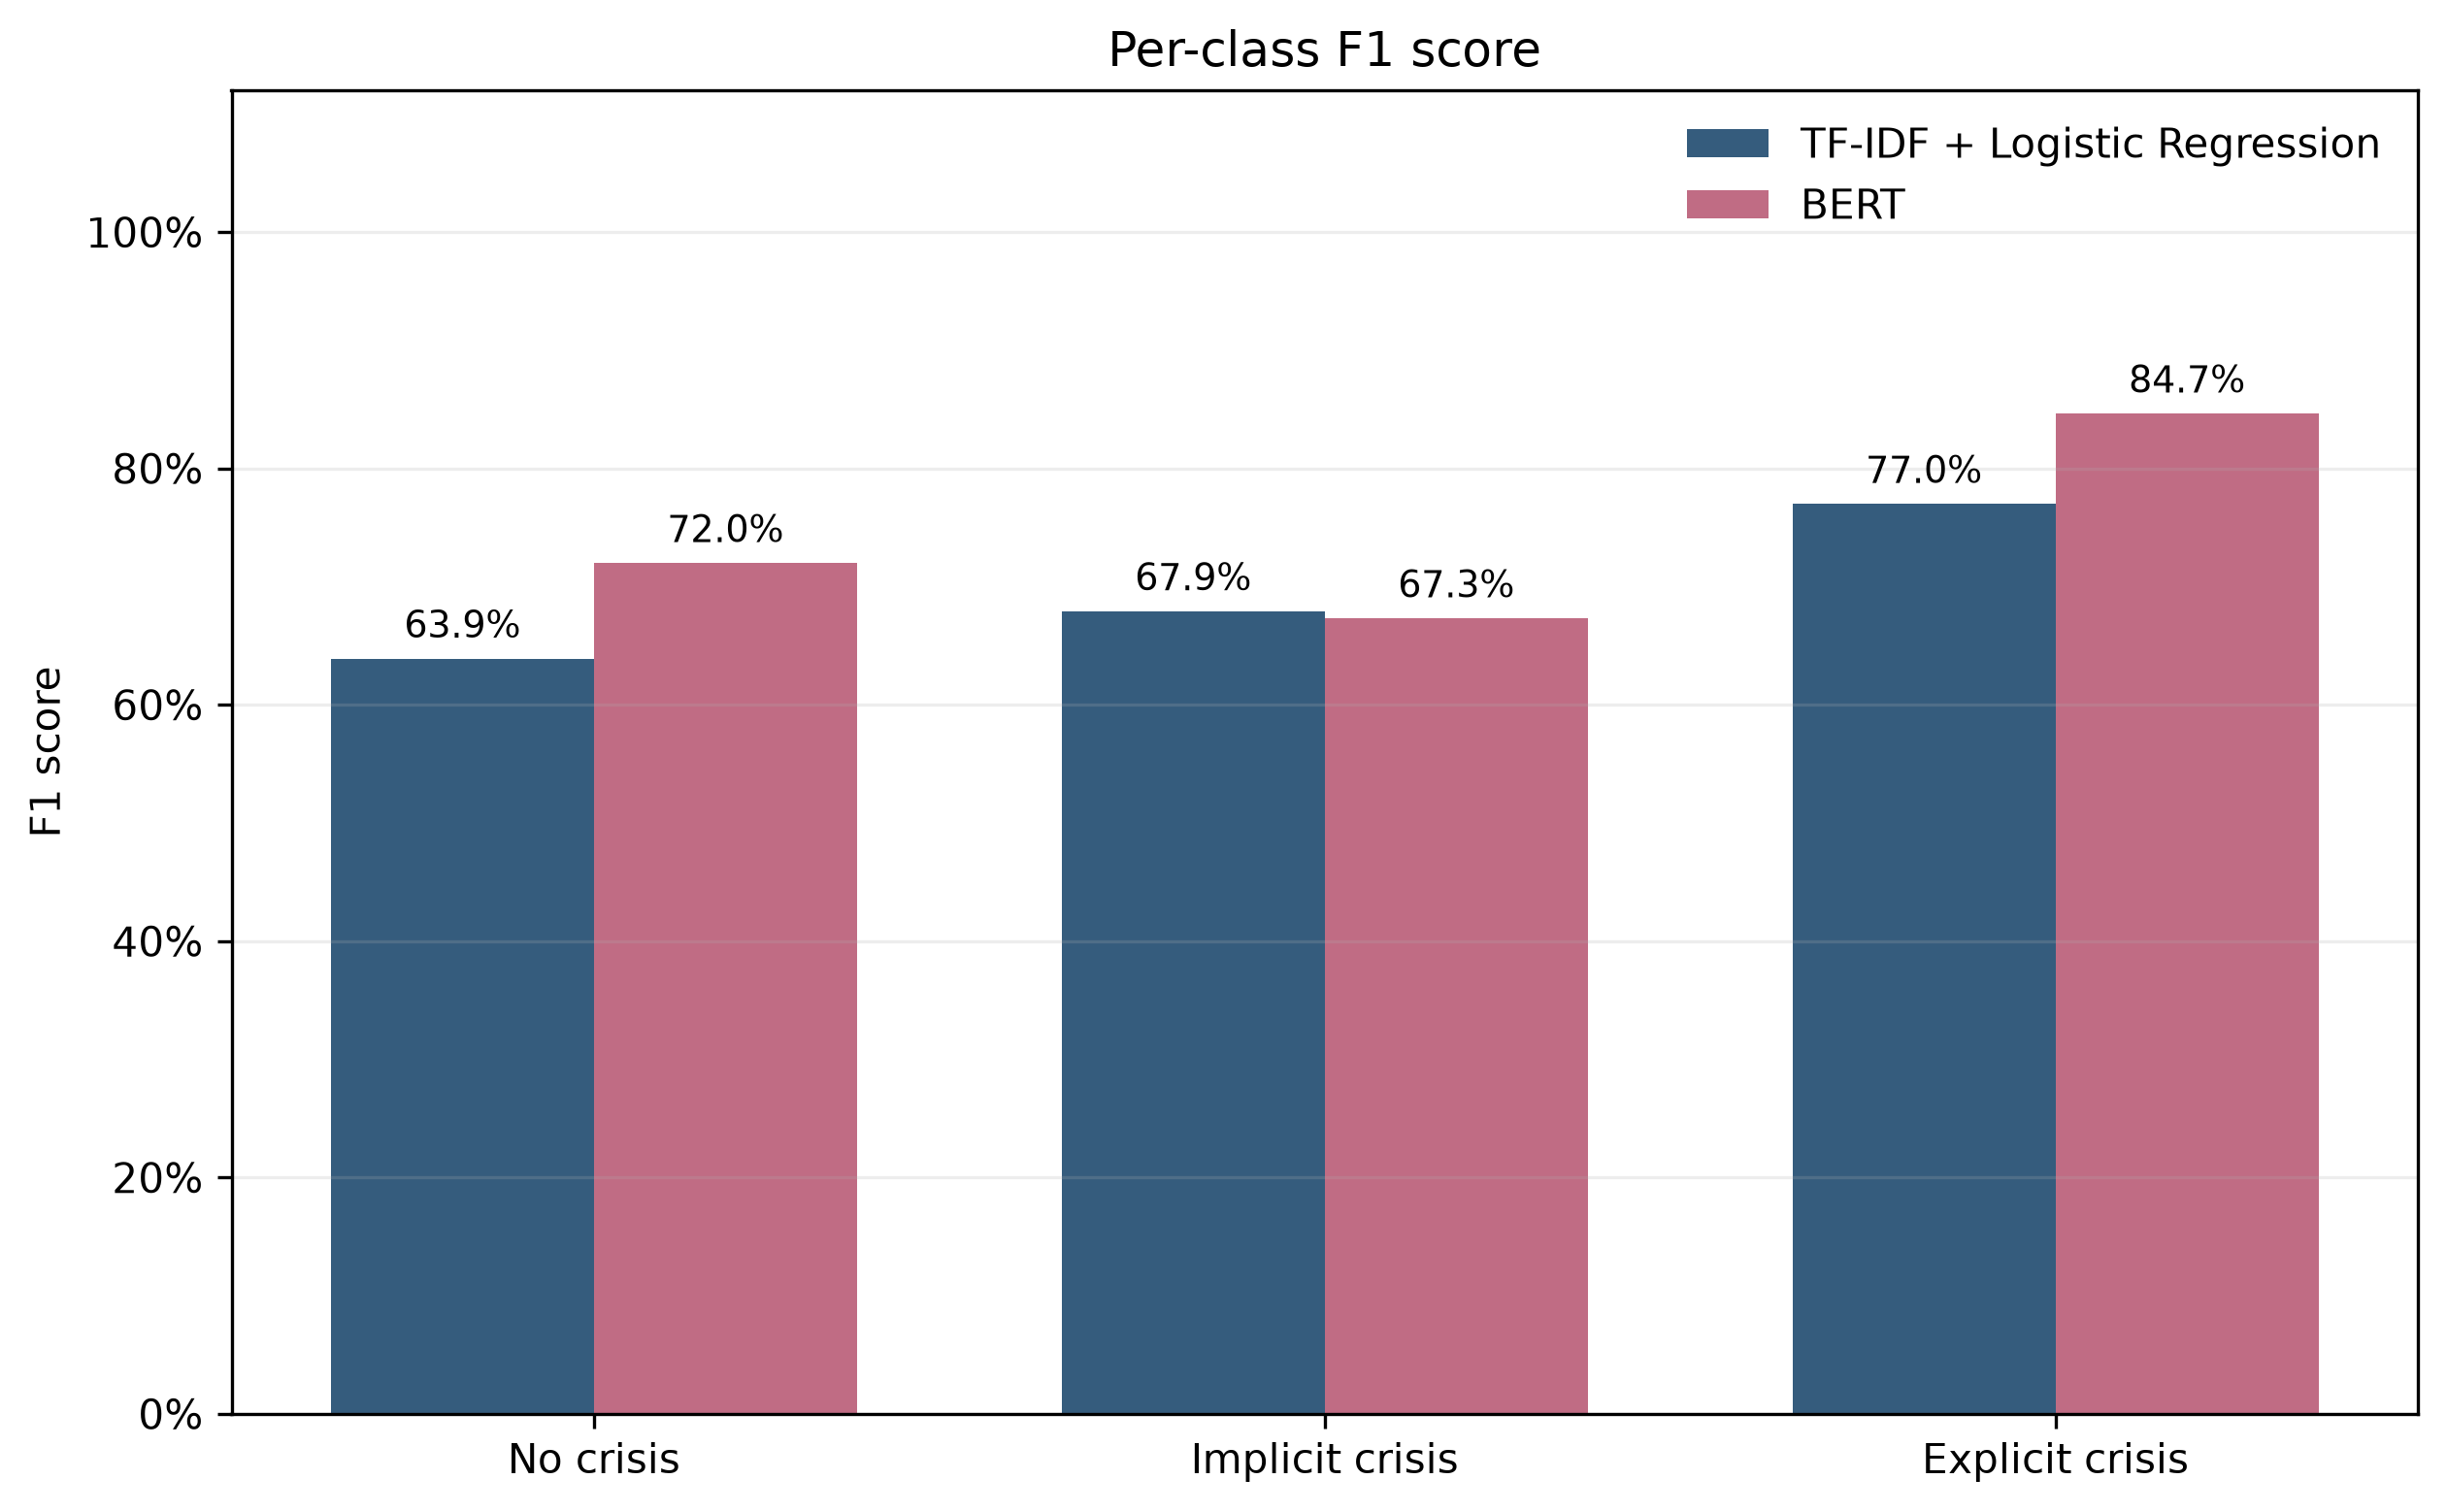
\includegraphics[width=0.8\textwidth]{per_class_f1.png}
\caption{Per-class F1 score for no-crisis, implicit-crisis, and explicit-crisis, by model.}
\label{fig:per-class-f1}
\end{figure}

BERT outperforms TF-IDF + Logistic Regression on the no-crisis class (72.00\% vs. 63.92\% F1) and, more substantially, on the explicit-crisis class (84.66\% vs. 77.01\% F1). On the implicit-crisis class, however, the two models are essentially tied, with TF-IDF marginally ahead: 67.92\% vs. 67.33\% F1, a difference of 0.59 percentage points on 49 test examples. This is the one result in this report that runs against the otherwise uniform pattern of BERT outperforming TF-IDF, and Section~\ref{sec:implicit-perf} discusses it in more detail.

\section{Confusion Matrix Analysis}

Figures~\ref{fig:cm-tfidf} and~\ref{fig:cm-bert} show the confusion matrices for TF-IDF + Logistic Regression and BERT, respectively; rows are true labels and columns are predicted labels, ordered no-crisis, implicit-crisis, explicit-crisis. Table~\ref{tab:cm-both} reproduces both matrices as a single table for direct side-by-side comparison.

\begin{figure}[H]
\centering
\begin{subfigure}[b]{0.48\textwidth}
\centering
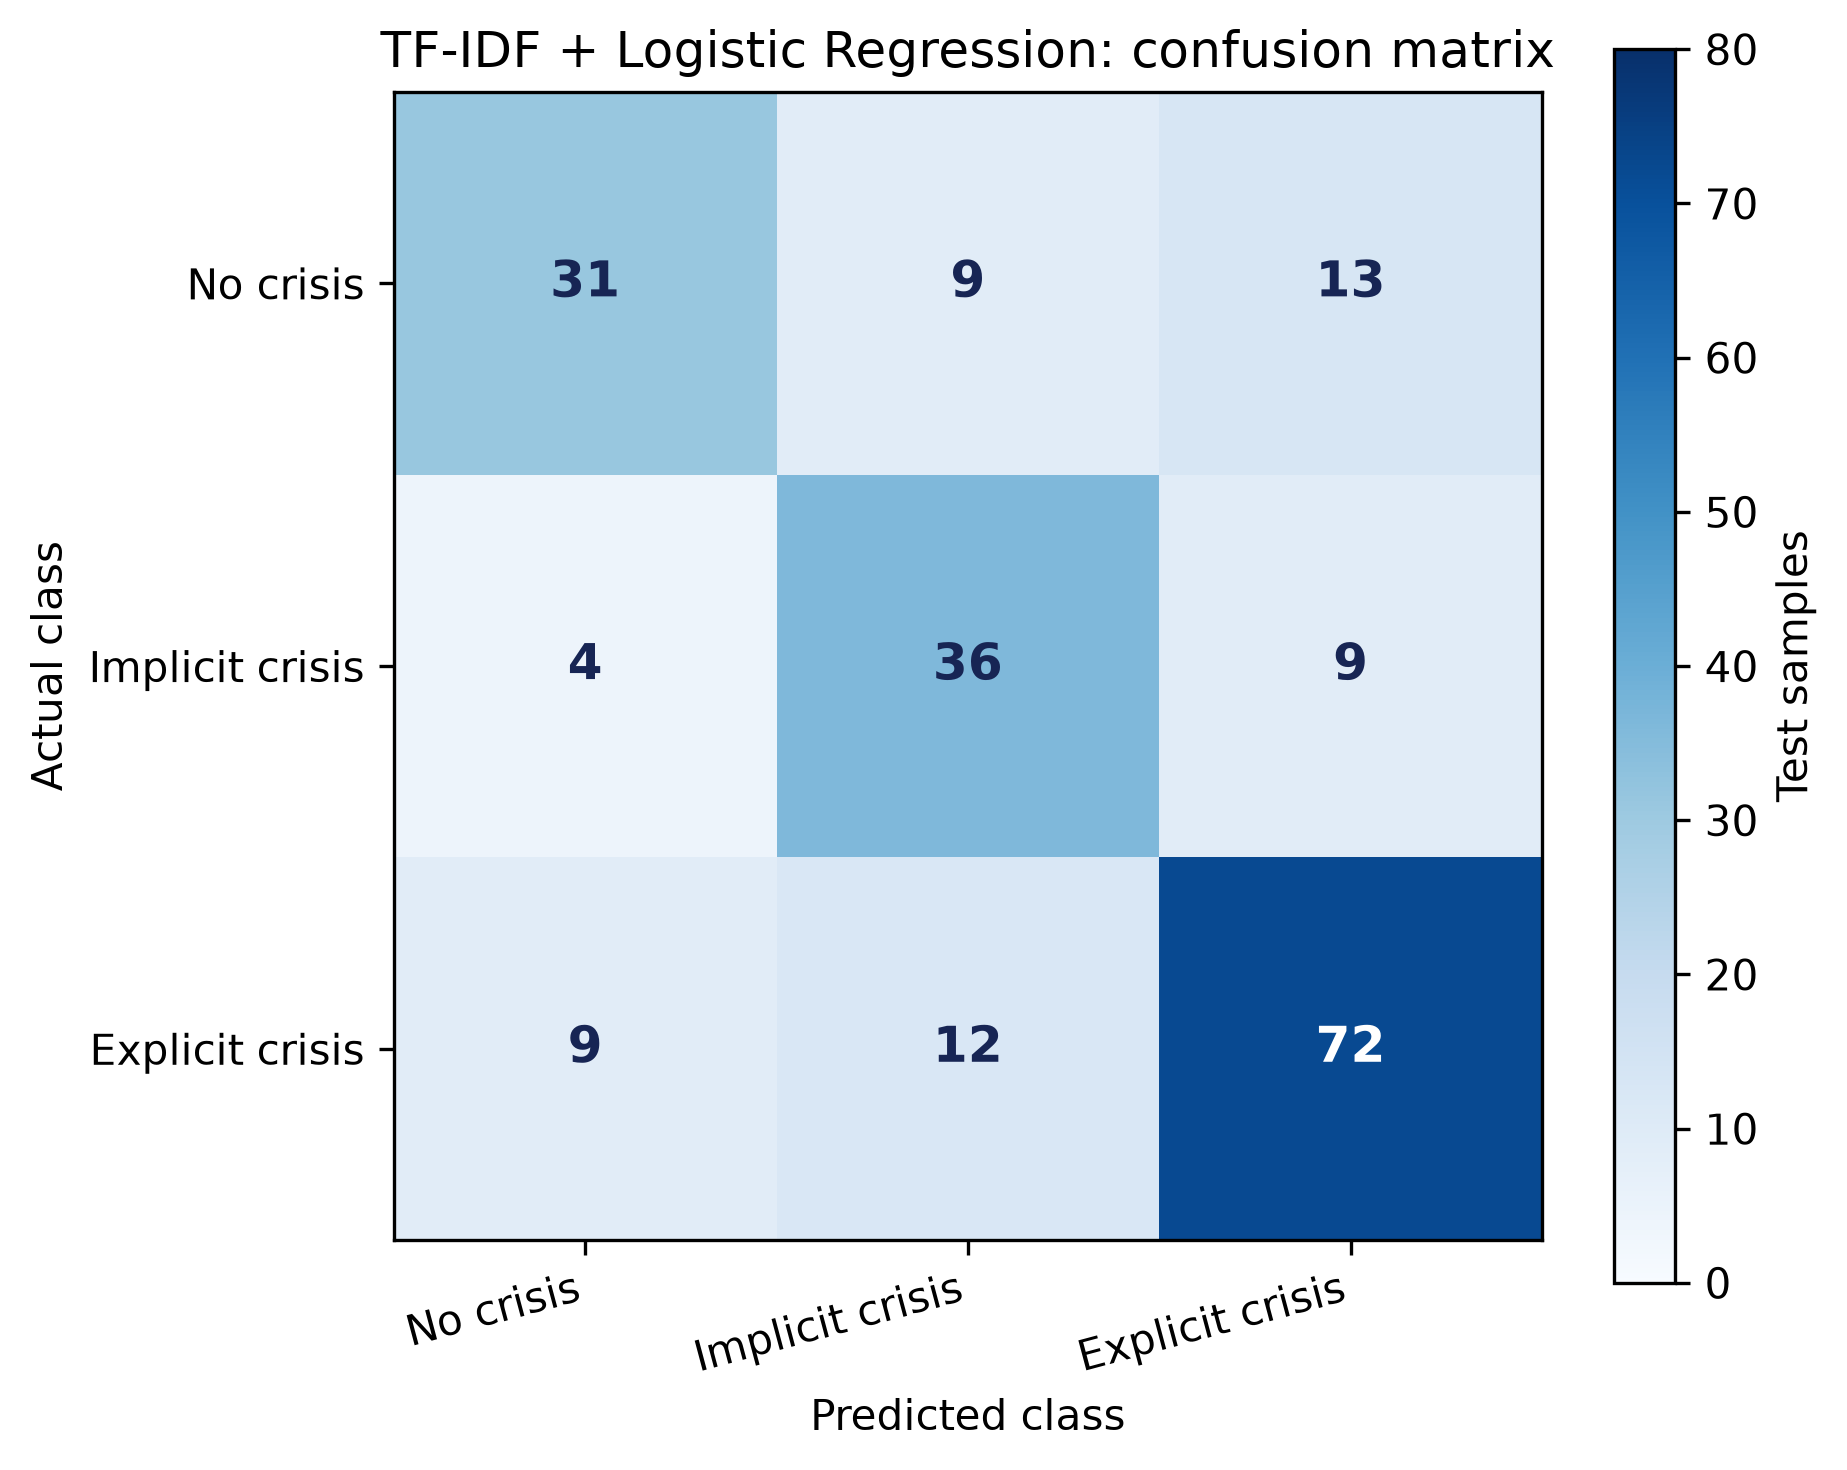
\includegraphics[width=\textwidth]{confusion_matrix_tfidf.png}
\caption{TF-IDF + Logistic Regression}
\label{fig:cm-tfidf}
\end{subfigure}
\hfill
\begin{subfigure}[b]{0.48\textwidth}
\centering
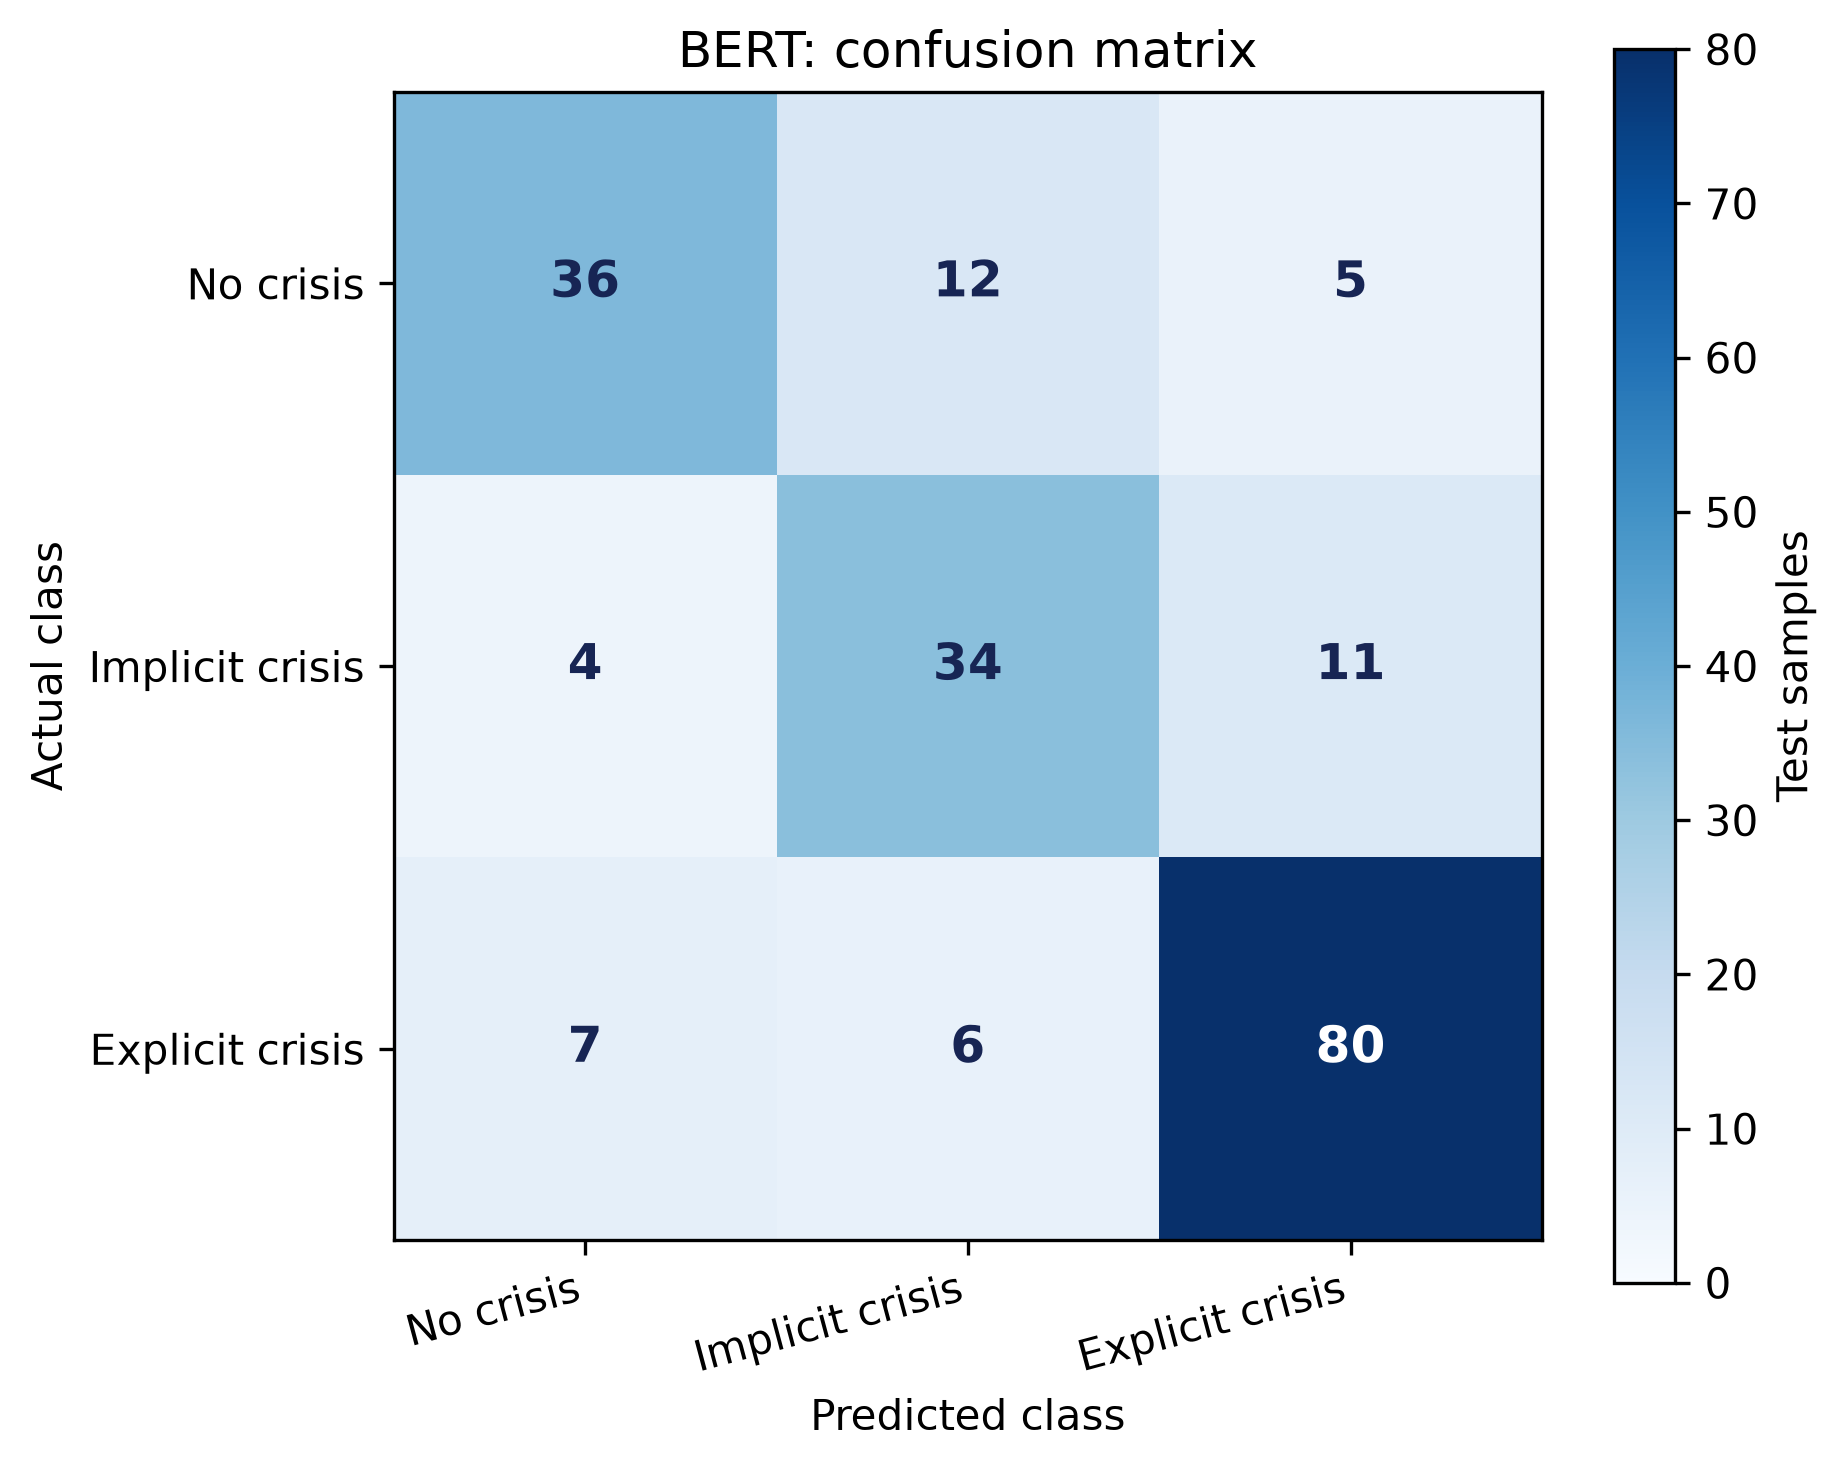
\includegraphics[width=\textwidth]{confusion_matrix_bert.png}
\caption{BERT}
\label{fig:cm-bert}
\end{subfigure}
\caption{Confusion matrices on the shared 195-row test set. Rows: true label. Columns: predicted label.}
\label{fig:confusion-matrices}
\end{figure}

\begin{table}[H]
\centering
\caption{Confusion matrix counts for both models (rows = actual, columns = predicted).}
\label{tab:cm-both}
\begin{tabular}{llrrr}
\toprule
\textbf{Model} & \textbf{Actual} & \textbf{Pred.\ No Crisis} & \textbf{Pred.\ Implicit} & \textbf{Pred.\ Explicit} \\
\midrule
\multirow{3}{*}{TF-IDF + LR}
 & No Crisis        & 31 & 9  & 13 \\
 & Implicit Crisis  & 4  & 36 & 9  \\
 & Explicit Crisis  & 9  & 12 & 72 \\
\midrule
\multirow{3}{*}{BERT}
 & No Crisis        & 36 & 12 & 5  \\
 & Implicit Crisis  & 4  & 34 & 11 \\
 & Explicit Crisis  & 7  & 6  & 80 \\
\bottomrule
\end{tabular}
\end{table}

Both models show the largest diagonal mass on explicit-crisis (TF-IDF: 72/93 correct; BERT: 80/93 correct), consistent with explicit-crisis being both the largest class and the class with the least ambiguity in its surface form. For the implicit-crisis row, both models make the same number of implicit$\rightarrow$no-crisis errors (4 each) but differ on implicit$\rightarrow$explicit errors (TF-IDF: 9; BERT: 11), meaning BERT is slightly more likely than TF-IDF to over-read implicit crisis language as explicit. For the no-crisis row, TF-IDF misclassifies 13 of 53 no-crisis examples as explicit-crisis, versus only 5 of 53 for BERT --- BERT is markedly less prone to this specific error, which is consistent with its higher no-crisis precision in Table~\ref{tab:per-class}.

\section{Implicit-Crisis Performance}
\label{sec:implicit-perf}

Implicit-crisis is the class this project is most concerned with, and it is also the class on which the two models are closest in performance. TF-IDF's implicit-crisis F1 (67.92\%) is driven by higher recall (73.47\% vs. BERT's 69.39\%) but lower precision (63.16\% vs. BERT's 65.38\%) than BERT; that is, TF-IDF recovers a slightly larger share of true implicit-crisis examples, at the cost of slightly more false positives from the other two classes. Given that this comparison is computed on only 49 test examples, the practical difference between the two models on this class should be read as \emph{approximately tied} rather than as a meaningful advantage for either model.

\section{Explicit-Crisis Performance}

Explicit-crisis is the class on which BERT shows its largest advantage: 84.66\% F1 versus TF-IDF's 77.01\%, a gap of 7.65 percentage points, driven by improvements in both precision (83.33\% vs. 76.60\%) and recall (86.02\% vs. 77.42\%). This is consistent with explicit-crisis language containing more directly interpretable lexical and contextual signal, which both a character-level lexical model and a contextual transformer can exploit, but which the transformer appears to exploit more effectively at this sample size.

\section{No-Crisis Performance}

BERT also outperforms TF-IDF on the no-crisis class (72.00\% vs. 63.92\% F1), driven primarily by higher recall (67.92\% vs. 58.49\%): TF-IDF misclassifies a larger share of genuinely non-crisis text as crisis-related (13 of 53 no-crisis examples predicted explicit-crisis, per Table~\ref{tab:cm-both}) than BERT does (5 of 53).

\section{Confidence Distribution}

Table~\ref{tab:confidence} and Figure~\ref{fig:confidence-dist} report confidence statistics computed over all 195 test predictions for each model.

\begin{table}[H]
\centering
\caption{Selected-class confidence statistics.}
\label{tab:confidence}
\begin{tabular}{lrr}
\toprule
\textbf{Statistic} & \textbf{TF-IDF + LR} & \textbf{BERT} \\
\midrule
Mean confidence   & 55.74\% & 94.60\% \\
Median confidence & 52.27\% & 99.28\% \\
Std.\ deviation   & 13.63\% & 10.14\% \\
Minimum           & 34.36\% & 53.55\% \\
Maximum           & 95.93\% & 99.75\% \\
\bottomrule
\end{tabular}
\end{table}

\begin{figure}[H]
\centering
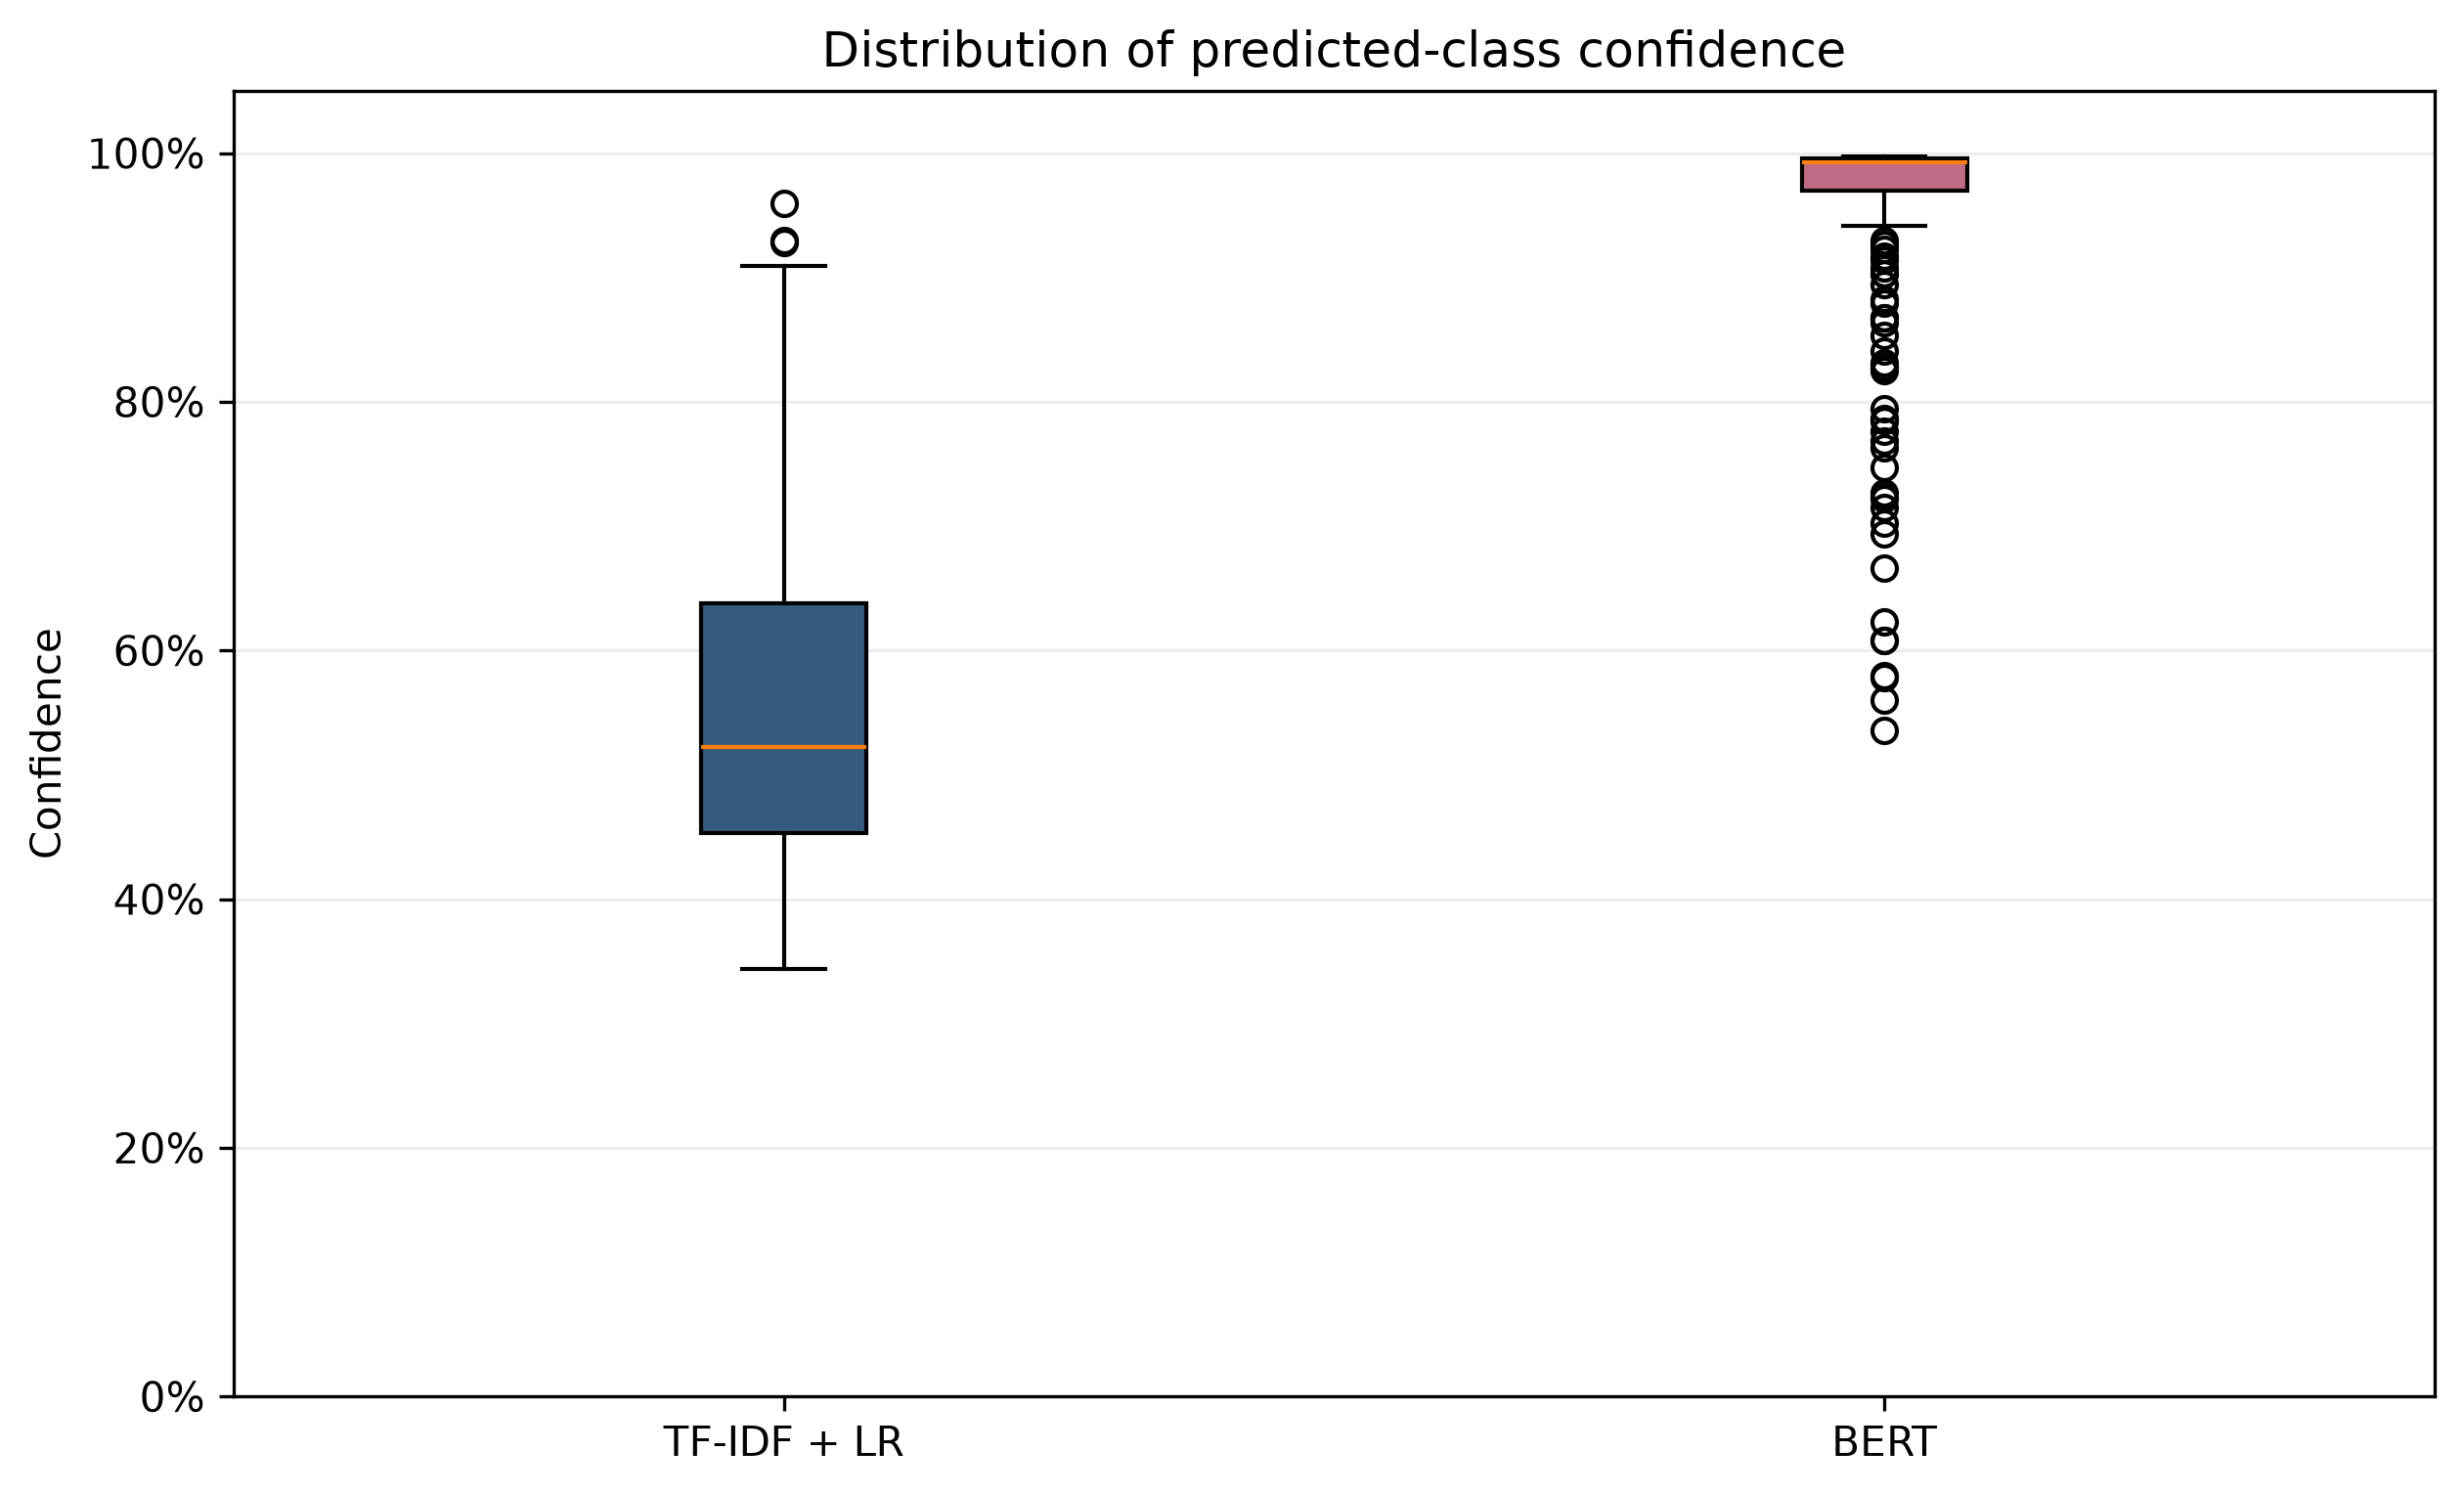
\includegraphics[width=0.8\textwidth]{confidence_distribution.png}
\caption{Distribution of selected-class confidence for TF-IDF + Logistic Regression and BERT.}
\label{fig:confidence-dist}
\end{figure}

BERT's confidence distribution is heavily concentrated near 1.0 (median 99.28\%), while TF-IDF's confidence is spread more broadly around its median of 52.27\%, reflecting the flatter probability distributions typically produced by a linear softmax classifier over sparse lexical features compared to a fine-tuned transformer. As established in Section~\ref{ch:methodology}, confidence is not accuracy: BERT's mean confidence of 94.60\% does not imply a 94.60\% accuracy rate, and its actual accuracy on this test set is 76.92\% (Table~\ref{tab:overall-metrics}).

\section{Calibration}

Table~\ref{tab:calibration} reports Expected Calibration Error for both models, and Figure~\ref{fig:calibration} shows the reliability diagram (observed accuracy versus mean confidence, per bin) alongside the diagonal line representing perfect calibration.

\begin{table}[H]
\centering
\caption{Expected Calibration Error (10 bins).}
\label{tab:calibration}
\begin{tabular}{lr}
\toprule
\textbf{Model} & \textbf{ECE} \\
\midrule
TF-IDF + LR & 0.1554 \\
BERT        & 0.1767 \\
\bottomrule
\end{tabular}
\end{table}

\begin{figure}[H]
\centering
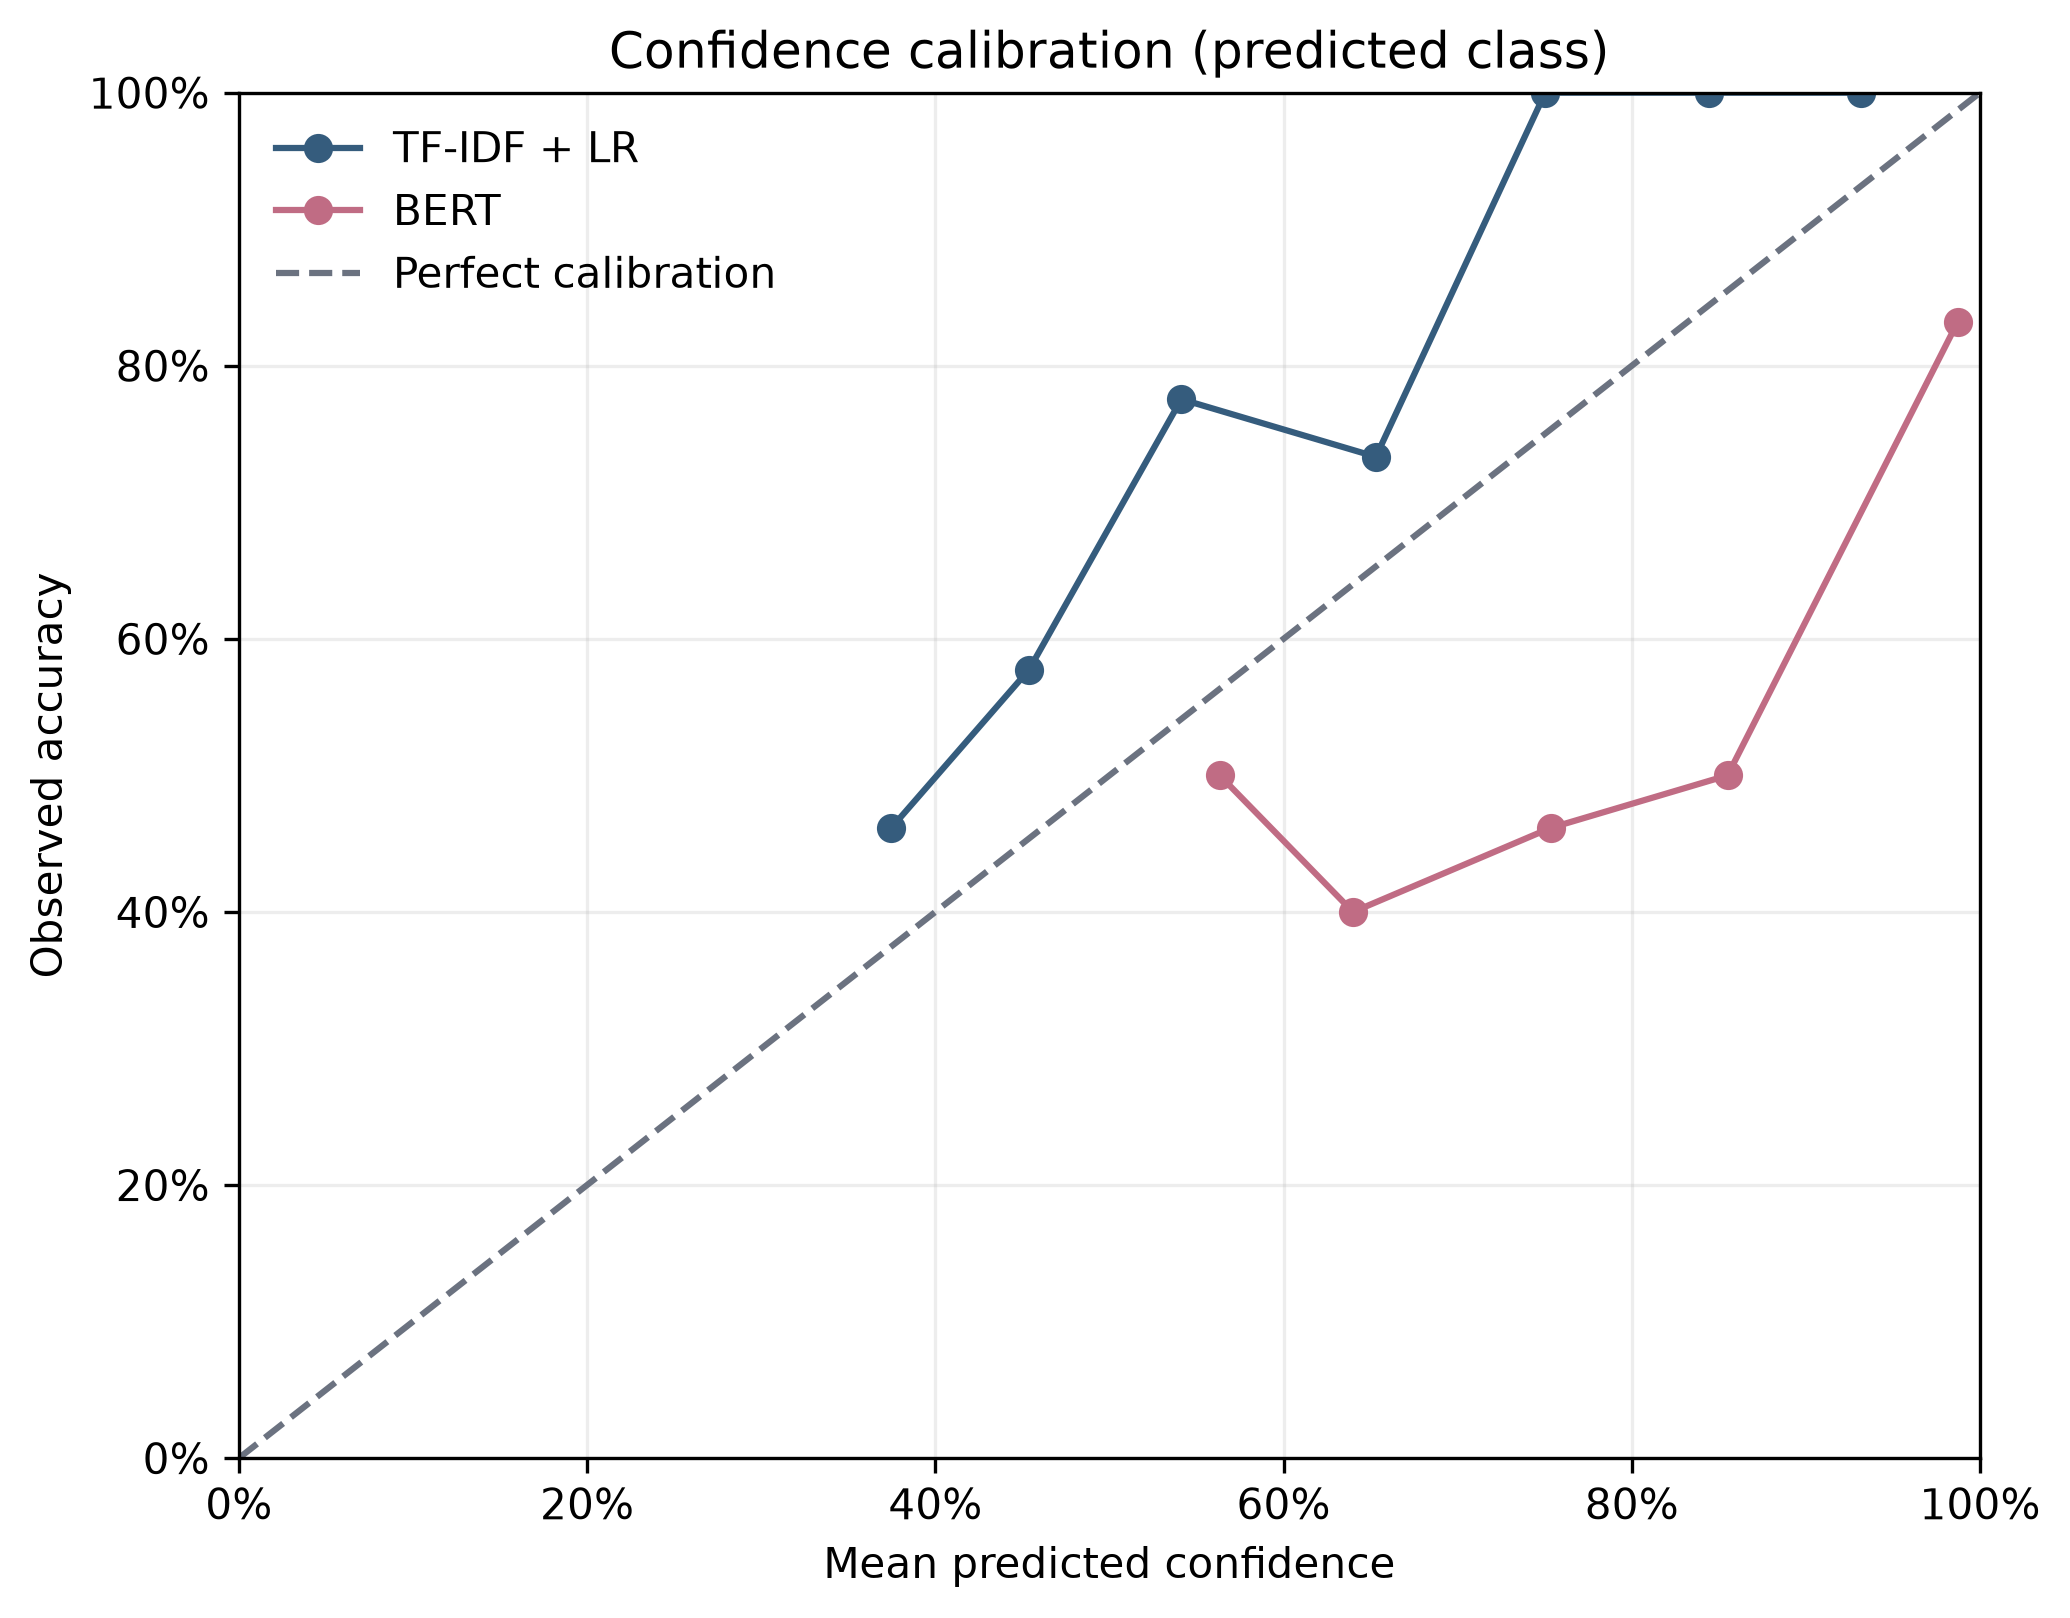
\includegraphics[width=0.7\textwidth]{calibration.png}
\caption{Reliability diagram: observed accuracy versus mean predicted confidence, per confidence bin, against the perfect-calibration diagonal.}
\label{fig:calibration}
\end{figure}

Despite having far higher average confidence, BERT has a \emph{higher} ECE than TF-IDF (0.1767 vs.\ 0.1554), meaning BERT's confidence values track its actual accuracy somewhat less faithfully than TF-IDF's do, on this test set. Given that BERT's mean confidence (94.60\%) sits well above its actual accuracy (76.92\%), the pattern in Figure~\ref{fig:calibration} is consistent with systematic overconfidence: BERT's predicted confidence exceeds its observed accuracy in its high-confidence bins. TF-IDF's confidence values are lower in absolute terms but sit closer to its own accuracy (71.28\%), which is reflected in its smaller ECE. Both models' calibration errors should be interpreted cautiously given the 195-row test size, which limits how many examples fall into each of the 10 calibration bins.

\section{Agreement and Disagreement}

Table~\ref{tab:agreement} and Figures~\ref{fig:agreement} and~\ref{fig:agreement-class} summarize where the two independent models select the same predicted class and where they diverge.

\begin{table}[H]
\centering
\caption{Model agreement on the 195-row test set.}
\label{tab:agreement}
\begin{tabular}{lrr}
\toprule
\textbf{Outcome} & \textbf{Count} & \textbf{Share} \\
\midrule
Agreement    & 148 & 75.9\% \\
Disagreement & 47  & 24.1\% \\
\bottomrule
\end{tabular}
\end{table}

\begin{figure}[H]
\centering
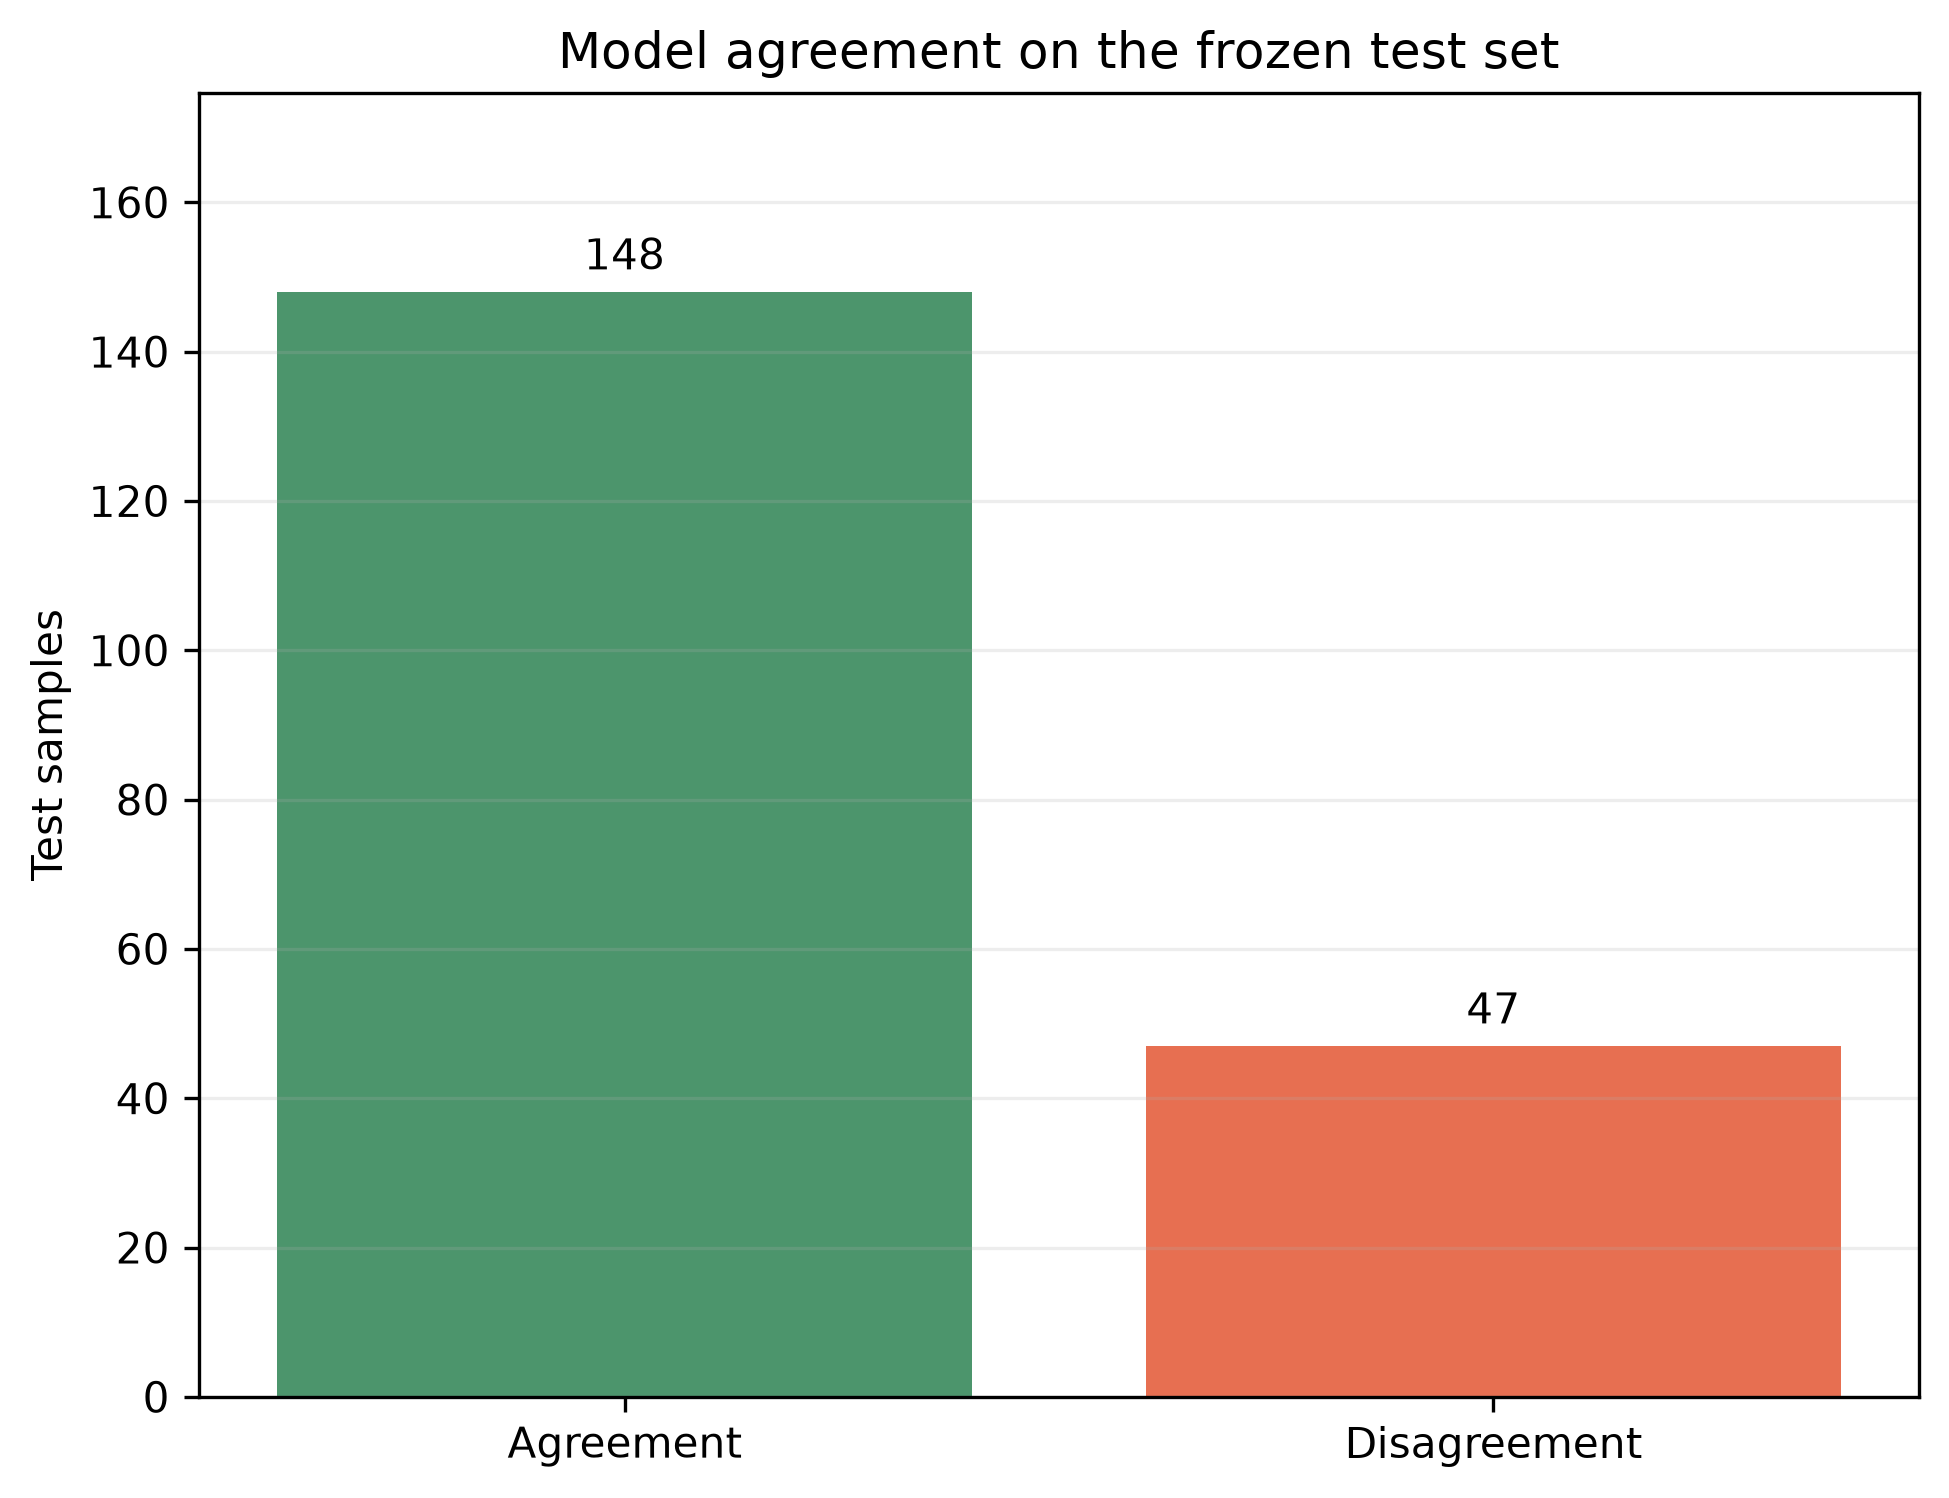
\includegraphics[width=0.65\textwidth]{model_agreement.png}
\caption{Overall count of test examples on which the two models' predicted labels agree versus disagree.}
\label{fig:agreement}
\end{figure}

\begin{figure}[H]
\centering
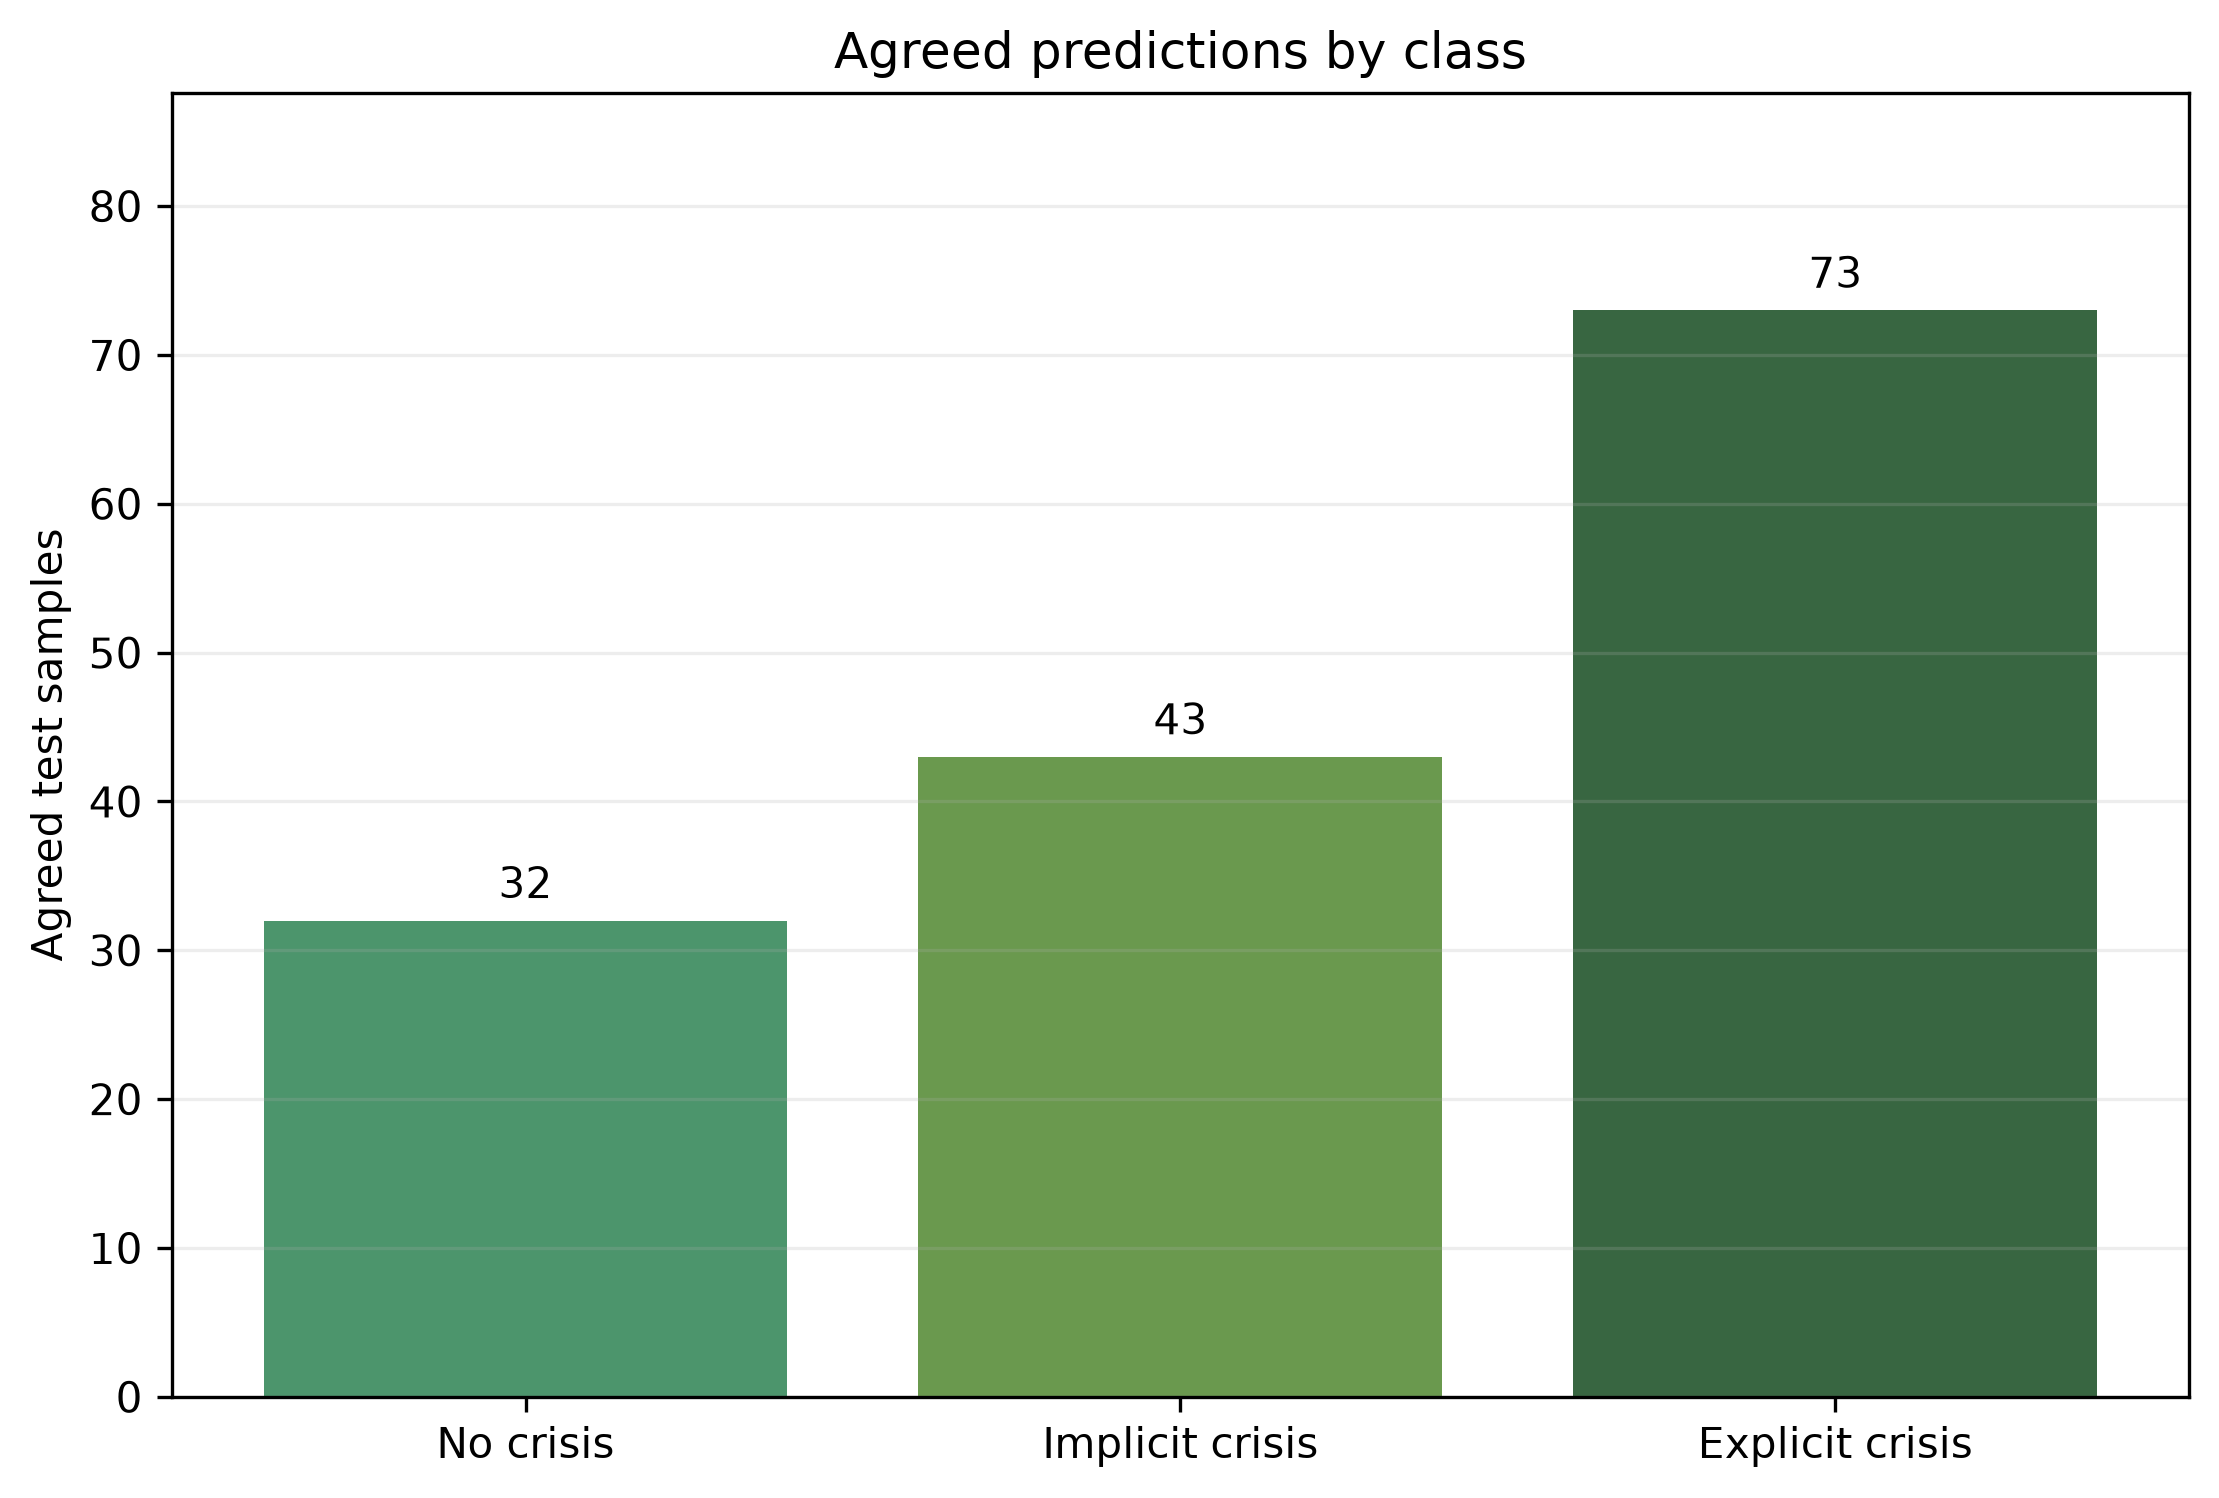
\includegraphics[width=0.8\textwidth]{agreement_by_class.png}
\caption{Class distribution among the shared (agreeing) predictions.}
\label{fig:agreement-class}
\end{figure}

Agreement means the two independently trained models selected the same numeric label; it says nothing about whether that shared label is correct. Of the 195 test rows, both models are correct on 124 (63.6\%), both are wrong on 30 (15.4\%), TF-IDF alone is correct on 15 (7.7\%), and BERT alone is correct on 26 (13.3\%). BERT is uniquely correct on roughly 1.7$\times$ as many examples as TF-IDF is uniquely correct on, which is broadly consistent with BERT's higher overall accuracy, but the existence of 15 examples that only TF-IDF gets right shows that the lexical model is not strictly subsumed by the transformer model on this test set.

\section{Confidence versus Correctness}

Figure~\ref{fig:conf-correct} groups confidence by model and by whether the prediction was correct, making it possible to see whether either model's confidence is a useful signal for distinguishing its own correct predictions from its own incorrect ones.

\begin{figure}[H]
\centering
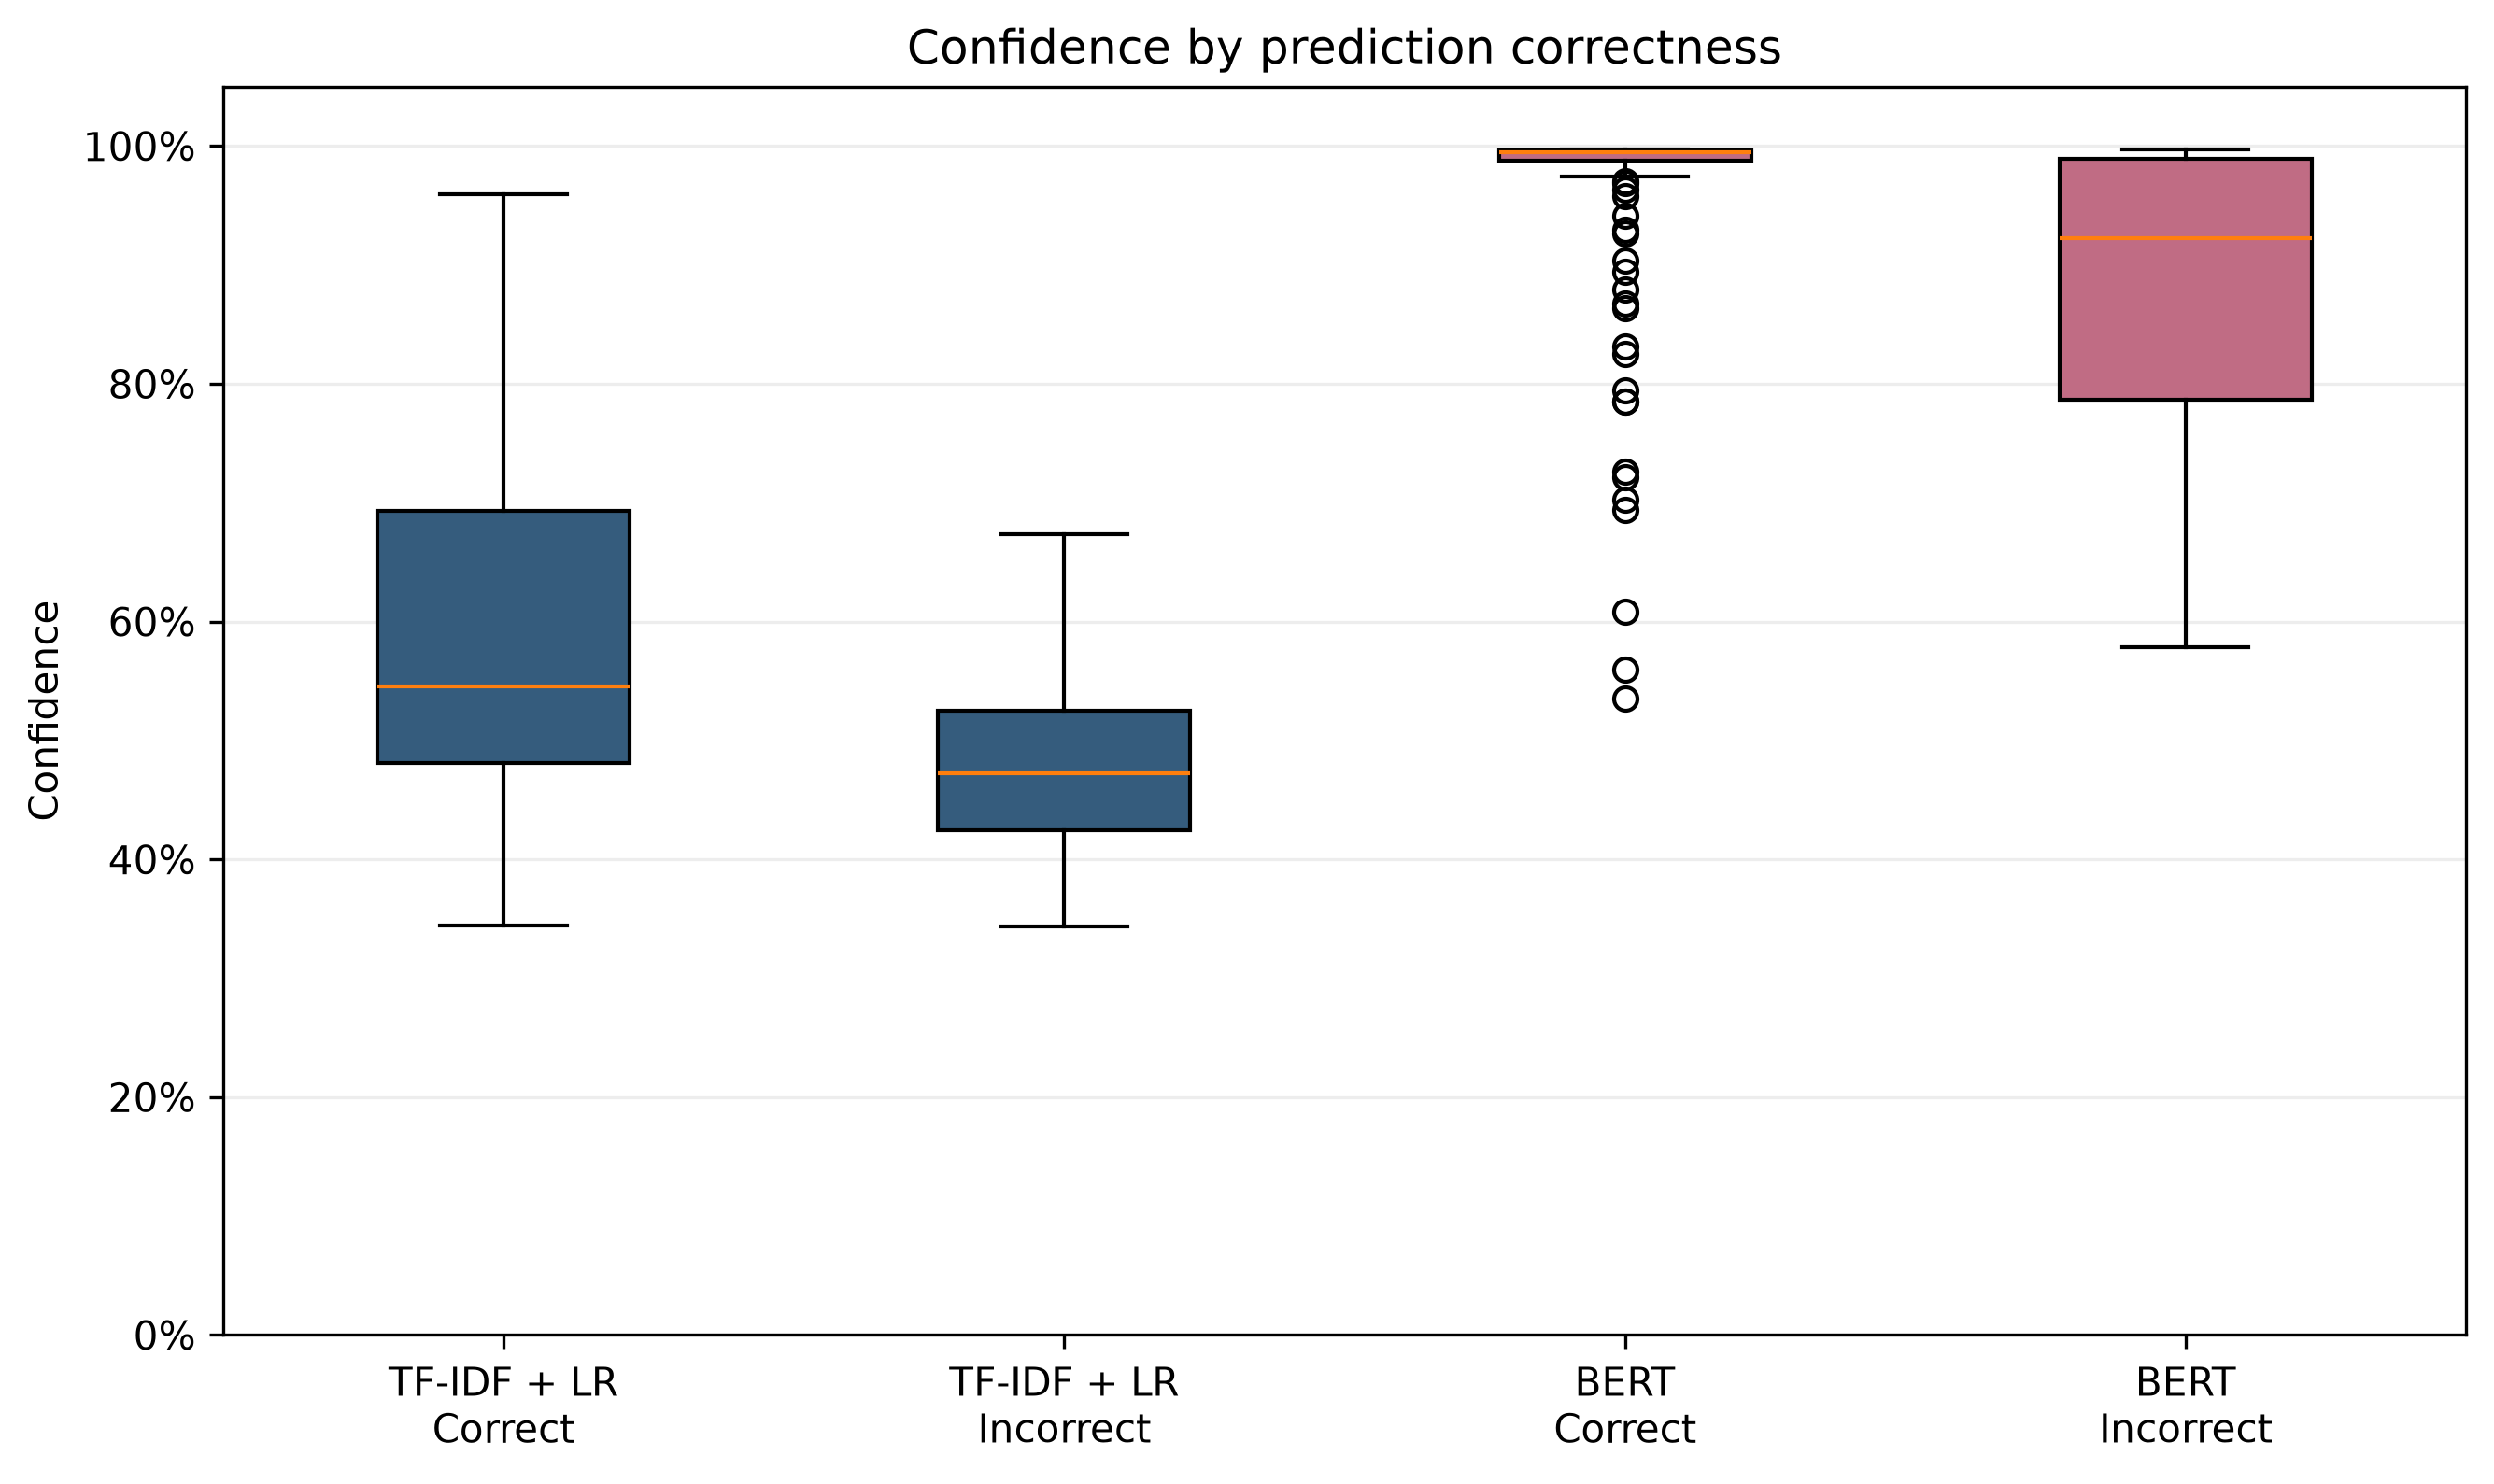
\includegraphics[width=0.8\textwidth]{confidence_vs_correctness.png}
\caption{Selected-class confidence, grouped by model and by prediction correctness.}
\label{fig:conf-correct}
\end{figure}

For both models, correct predictions tend to carry higher confidence than incorrect ones, which is the expected direction for a usable confidence signal. However, because BERT's confidence distribution is compressed near 1.0 even for many of its incorrect predictions (consistent with its higher ECE in Table~\ref{tab:calibration}), a fixed high-confidence threshold on BERT's output would still pass through a non-trivial share of wrong answers; TF-IDF's more spread confidence distribution makes its confidence value comparatively more informative as a per-example correctness signal, even though its overall accuracy is lower.

\section{Detailed Error Analysis}

An aggregate error analysis was performed directly on \texttt{results/\pbrk model\_\pbrk comparison/\pbrk predictions.csv} (195 rows) to characterize where and how the two models' errors overlap or diverge, without reproducing individual crisis-related message text.

\begin{itemize}[nosep]
  \item \textbf{Both models correct}: 124 of 195 (63.6\%).
  \item \textbf{Both models wrong}: 30 of 195 (15.4\%) --- cases neither representation handles correctly on this test set.
  \item \textbf{TF-IDF correct, BERT wrong}: 15 of 195 (7.7\%).
  \item \textbf{BERT correct, TF-IDF wrong}: 26 of 195 (13.3\%).
  \item \textbf{Model disagreement}: 47 of 195 (24.1\%), matching Table~\ref{tab:agreement}.
  \item \textbf{No-crisis $\rightarrow$ explicit-crisis errors}: TF-IDF makes this error on 13 of 53 no-crisis examples; BERT makes it on 5 of 53. This is the single largest source of TF-IDF's no-crisis precision gap relative to BERT.
  \item \textbf{Explicit-crisis $\rightarrow$ no-crisis errors}: TF-IDF makes this error on 9 of 93 explicit-crisis examples; BERT makes it on 7 of 93 --- both models occasionally miss clearly-worded crisis language entirely, at broadly similar rates.
  \item \textbf{Implicit-crisis confusion}: both models confuse implicit-crisis with no-crisis at the same rate (4 of 49 each); TF-IDF confuses implicit-crisis with explicit-crisis slightly less often than BERT does (9 of 49 vs.\ 11 of 49).
\end{itemize}

The pattern that emerges is not that one model is strictly superior: BERT more effectively separates no-crisis from explicit-crisis text, but the two models are essentially interchangeable on the implicit-crisis class, and each model correctly classifies a non-overlapping subset of examples that the other model gets wrong (15 TF-IDF-only-correct vs.\ 26 BERT-only-correct), which is consistent with the two models drawing on structurally different signal (character-level lexical patterns vs.\ contextual meaning) rather than one model simply being a strictly better version of the other.

\chapter{Discussion}

\section{Overall Comparison}

On the frozen 195-sample evaluation set, BERT achieved higher overall accuracy and macro-F1 than TF-IDF + Logistic Regression, while TF-IDF + Logistic Regression produced a slightly higher F1 score for the implicit-crisis class specifically. Neither model is uniformly superior across every axis reported in Chapter~\ref{ch:results}: BERT leads on aggregate accuracy, macro metrics, no-crisis F1, and explicit-crisis F1; TF-IDF leads (marginally) on implicit-crisis F1 and is better calibrated relative to its own confidence. The correct framing of this project's central result is therefore comparative and class-conditional, not a single "which model wins" verdict.

\section{TF-IDF Strengths}

TF-IDF + Logistic Regression is markedly cheaper to run (sparse linear operations on CPU vs.\ a 12-layer transformer forward pass), produces a confidence distribution that is more spread out and, by ECE, somewhat closer to its own accuracy, and is not meaningfully behind BERT on the implicit-crisis class specifically. Its character-level representation also means it degrades gracefully on misspelled or non-standard text without any separate spelling-correction stage, since character n-grams remain partially matchable even under spelling variation.

\section{BERT Strengths}

BERT's advantage is concentrated in the classes with more explicit surface signal: it substantially outperforms TF-IDF on explicit-crisis F1 (84.66\% vs.\ 77.01\%) and reduces the specific error of misclassifying non-crisis text as explicit-crisis (5 of 53 vs.\ TF-IDF's 13 of 53). Its contextual representation appears to help most where the classification decision benefits from understanding the sentence as a whole, rather than from matching sub-word lexical patterns.

\section{Implicit-Crisis Detection}

Implicit-crisis is, by construction, the class where crisis intent is not stated directly, and it is the class both models handle worst relative to their own explicit-crisis performance (TF-IDF: 67.92\% vs.\ 77.01\%; BERT: 67.33\% vs.\ 84.66\%). That BERT's additional contextual modeling capacity does not translate into a clear implicit-crisis advantage over the much simpler TF-IDF baseline is the most notable finding of this comparison: it suggests that, at least on this 49-example test slice, the gap between implicit and explicit crisis language is not primarily a gap that more contextual representational power alone closes. This is consistent with implicit expression depending on pragmatic or situational inference that neither model's training signal may sufficiently capture, rather than a limitation specific to one representation.

\section{Explicit-Crisis Detection}

The explicit-crisis result is the cleanest evidence in this report that BERT's contextual representation provides a genuine advantage on this dataset: the gap (7.65 F1 points) is the largest of the three per-class gaps, is driven by improvements in both precision and recall, and appears on the largest of the three test classes (93 examples), giving it more statistical weight than the implicit-crisis comparison.

\section{Confidence and Calibration}

BERT's much higher mean confidence (94.60\% vs.\ 55.74\%) together with its higher ECE (0.1767 vs.\ 0.1554) is a specific and important combination: it means BERT is not simply "more confident because it is more accurate" — its confidence outpaces its accuracy by a wider margin than TF-IDF's confidence outpaces its accuracy. Any downstream use of these models' confidence scores (for example, to flag low-confidence predictions for human review) would need model-specific confidence thresholds, since a fixed threshold interpreted the same way for both models would not carry the same reliability guarantee for each.

\section{Model Disagreement}

The two models disagree on 24.1\% of test examples (47 of 195), and disagreement is not evenly distributed across correctness outcomes: BERT is uniquely correct on 26 examples where TF-IDF is wrong, while TF-IDF is uniquely correct on 15 examples where BERT is wrong. This asymmetry, combined with the existence of 30 examples both models get wrong, indicates that model disagreement, on its own, is not a reliable proxy for "the more sophisticated model must be right" --- in roughly a third of disagreement cases, the simpler lexical model is the one that gets the example correct.

\section{Practical Interpretation}

Taken together, these results support presenting both models' predictions side by side, as CrisisSense's frontend does, rather than treating either model in isolation as a ground-truth signal, and rather than combining them into a single ensemble score that would obscure exactly the class-conditional and confidence-conditional differences documented in Chapter~\ref{ch:results}. A practitioner interested specifically in implicit-crisis recall should not assume that deploying only the larger, higher-accuracy model is sufficient; the evidence here suggests the two models are close to interchangeable on that specific class.

\section{What the Results Do and Do Not Show}

These results show: (1) BERT's higher accuracy and macro-F1 on this specific 195-row test set; (2) an approximate tie between the two models on implicit-crisis F1 on this test set; (3) that BERT's much higher confidence is accompanied by somewhat worse calibration, not better; and (4) that model agreement does not imply correctness for either model. These results do \emph{not} show that BERT is unconditionally better than TF-IDF at implicit-crisis detection, that either model generalizes to different text domains or platforms beyond this dataset, that either model's confidence score can be used directly as a calibrated probability of correctness without further calibration work, or that either model is suitable for any form of individual-level clinical or risk assessment. Every quantitative claim in this report is scoped to the 195-sample frozen test set on which it was measured.

\chapter{Limitations}
\label{ch:limitations}

The following limitations are directly supported by the current project documentation and the evaluation artifacts examined in this report.

\begin{itemize}[nosep,leftmargin=*]
  \item \textbf{Small test set.} All results in Chapter~\ref{ch:results} are computed on a single 195-sample frozen test set. Metrics computed at this scale, particularly per-class metrics, carry meaningful statistical uncertainty, and small differences (such as the 0.59-point implicit-crisis F1 gap) should not be over-interpreted as robust, generalizable effects.

  \item \textbf{Small implicit-crisis subclass.} The implicit-crisis class --- the class most central to this project's motivation --- has only 49 test examples, the smallest of the three classes. Conclusions about implicit-crisis performance rest on the narrowest evidentiary base in this report.

  \item \textbf{Model disagreement.} The two models disagree on 24.1\% of test examples. This report does not resolve which model is correct in a disagreement case without reference to the ground-truth label, and no automated arbitration mechanism between the two models exists in the deployed system.

  \item \textbf{Calibration limitations.} Both models exhibit non-trivial Expected Calibration Error (TF-IDF: 0.155; BERT: 0.177), and BERT in particular shows a pattern consistent with overconfidence. Neither model's raw softmax probability should be treated as a calibrated estimate of the true probability of correctness.

  \item \textbf{Confidence interpretation.} Confidence values are not directly comparable across the two models: BERT's confidence distribution is compressed near 1.0 regardless of correctness to a greater degree than TF-IDF's, so the same numeric confidence threshold does not carry equivalent meaning for both models.

  \item \textbf{Frozen artifacts.} Both models are frozen inference-only artifacts in the current deployed system. The BERT model's original fine-tuning process is not re-executed or re-verified as part of this report; the evaluation in Chapter~\ref{ch:results} describes the behavior of the already-trained, saved artifact, not a reproduction of its training procedure.

  \item \textbf{Dataset scope.} The dataset underlying the frozen splits (1{,}294 rows total) is fixed and was not expanded or re-annotated for this report. Its source domain, collection process, and original annotation methodology are documented only to the extent recorded in the frozen split provenance files; deeper annotation-quality claims are outside the scope of what the current runtime artifacts can verify.

  \item \textbf{Not a clinical tool.} CrisisSense performs text classification. It does not diagnose individuals, does not clinically assess suicide risk, does not determine whether a person will attempt self-harm, and does not replace professional assessment or provide medical advice. No claim in this report should be read as a clinical-effectiveness claim.

  \item \textbf{Generalization.} Both models were trained and evaluated on the same fixed dataset distribution. Their performance on text drawn from different platforms, writing styles, languages, or time periods than those represented in the current dataset is untested and should not be assumed to match the results reported here.
\end{itemize}

\chapter{Conclusion}

This report documented CrisisSense, a frozen three-class crisis-language classification system that runs a character-level TF-IDF + Logistic Regression model and a BERT sequence-classification model independently on submitted text, without combining their outputs into an ensemble. Both models were evaluated on an identical, frozen 195-row test set drawn from a 1{,}294-row dataset split 905/194/195 into train/validation/test.

On this shared test set, BERT achieved higher overall accuracy (76.92\% vs.\ 71.28\%) and macro-F1 (74.66\% vs.\ 69.62\%) than TF-IDF + Logistic Regression, and a substantially higher F1 on the explicit-crisis class (84.66\% vs.\ 77.01\%). On the implicit-crisis class specifically, the two models were essentially tied, with TF-IDF marginally ahead (67.92\% vs.\ 67.33\% F1). BERT's mean selected-class confidence (94.60\%) was far higher than TF-IDF's (55.74\%), but this was accompanied by a higher Expected Calibration Error (0.177 vs.\ 0.155), not a lower one, indicating that BERT's higher confidence does not correspond to proportionally higher reliability on this test set. The two models agreed on 75.9\% of test predictions and disagreed on 24.1\%; agreement was shown to correlate with, but not guarantee, correctness for either model.

This project demonstrates that overall accuracy and macro-F1 do not tell the whole story of a model comparison: a model that leads clearly in aggregate metrics can still be matched, on a specific and practically important subclass, by a much simpler and cheaper baseline. It also demonstrates that a large gap in reported confidence between two models is not evidence that the more confident model is more trustworthy, once that confidence is checked against calibration error rather than taken at face value. CrisisSense classifies crisis-related language in text; it does not diagnose individuals, does not assess suicide risk, and its results in this report are scoped strictly to the frozen 195-sample evaluation set on which they were measured.

\chapter{Future Work}

The following directions are grounded in the current system's documented limitations (Chapter~\ref{ch:limitations}) and are distinguished explicitly from the work already completed and reported in Chapter~\ref{ch:results}.

\begin{itemize}[nosep,leftmargin=*]
  \item \textbf{Larger evaluation sets.} Expanding the frozen test set, or constructing an additional held-out evaluation set, would narrow the statistical uncertainty around the per-class metrics reported here, particularly for the 49-example implicit-crisis class.

  \item \textbf{Broader domain coverage.} Evaluating both frozen models on text drawn from additional platforms, writing styles, or time periods than those represented in the current dataset would test whether the results in Chapter~\ref{ch:results} generalize beyond the current fixed distribution.

  \item \textbf{Improved implicit-crisis data.} Given that implicit-crisis is both the smallest class and the class on which neither model shows a clear advantage, targeted collection or annotation of additional implicit-crisis examples is a direct way to both improve statistical confidence in this class's metrics and give future model training more signal on the harder, more indirect end of the label scheme.

  \item \textbf{Additional validation.} Independent re-annotation or inter-annotator agreement studies on a sample of the dataset would strengthen claims about label quality that the current runtime artifacts alone cannot verify.

  \item \textbf{Calibration methods.} Post-hoc calibration techniques (for example, temperature scaling or isotonic regression) applied to BERT's output probabilities could be explored to reduce its Expected Calibration Error without altering its underlying predictions, making its confidence scores more directly usable as a correctness signal.

  \item \textbf{Error-focused data collection.} The aggregate error analysis in Section~\ref{sec:per-class-results} and Chapter~\ref{ch:results} identified specific, recurring error patterns (notably no-crisis $\rightarrow$ explicit-crisis for TF-IDF, and implicit-crisis $\rightarrow$ explicit-crisis for both models); collecting or annotating additional examples that specifically probe these confusion patterns is a more targeted alternative to indiscriminate dataset expansion.

  \item \textbf{External and generalization testing.} Testing both models against text from a genuinely external source, not derived from the current dataset's collection process, would be needed before drawing any conclusion about real-world deployment performance.

  \item \textbf{Model fine-tuning improvements.} Future work could explore re-fine-tuning the BERT model with calibration-aware training objectives or class-balanced sampling, to test whether its implicit-crisis performance and calibration can be improved without sacrificing its current explicit-crisis and no-crisis advantages.
\end{itemize}

None of the directions above have been implemented in the current frozen system; they are proposed next steps, not claims about work already completed.


\bibliographystyle{plain}
\bibliography{references}

\appendix
\chapter{Current Project Structure}

\begin{lstlisting}
.
|-- backend/                         # FastAPI inference
|-- data/final_datasets/splits/      # current frozen copies
|-- models/{bert_no_severity,tfidf_logistic_regression}/
|-- results/model_comparison/        # current metrics and figures
|-- scripts/{data,evaluate_current_models.py}
|-- tests/test_inference_api.py
|-- New_docs/
|   |-- CRISISSENSE_CURRENT_PROJECT.md
|   `-- architecture/                # Mermaid and PNG diagrams
|-- index.html
|-- requirements.txt
|-- requirements-ml.txt
`-- README.md
\end{lstlisting}

\chapter{API Response Format}

Example \texttt{POST /\pbrk predict} request body:
\begin{lstlisting}
{
  "text": "I feel exhausted and cannot see a way forward."
}
\end{lstlisting}

Example response body (illustrative structure; probability values are per-request):
\begin{lstlisting}
{
  "text": "I feel exhausted and cannot see a way forward.",
  "tfidf": {
    "label": 1,
    "class_name": "implicit_crisis",
    "probabilities": {
      "no_crisis": 0.21,
      "implicit_crisis": 0.52,
      "explicit_crisis": 0.27
    }
  },
  "bert": {
    "label": 1,
    "class_name": "implicit_crisis",
    "probabilities": {
      "no_crisis": 0.05,
      "implicit_crisis": 0.88,
      "explicit_crisis": 0.07
    }
  }
}
\end{lstlisting}

\chapter{Additional Metrics}

\begin{table}[H]
\centering
\caption{Confidence-versus-correctness summary (derived from \texttt{predictions.csv}).}
\begin{tabular}{lrr}
\toprule
\textbf{Outcome} & \textbf{Count} & \textbf{Share of 195} \\
\midrule
Both models correct       & 124 & 63.6\% \\
Both models wrong         & 30  & 15.4\% \\
TF-IDF correct, BERT wrong & 15 & 7.7\%  \\
BERT correct, TF-IDF wrong & 26 & 13.3\% \\
\bottomrule
\end{tabular}
\end{table}

\chapter{Additional Figures}

\begin{figure}[H]
\centering
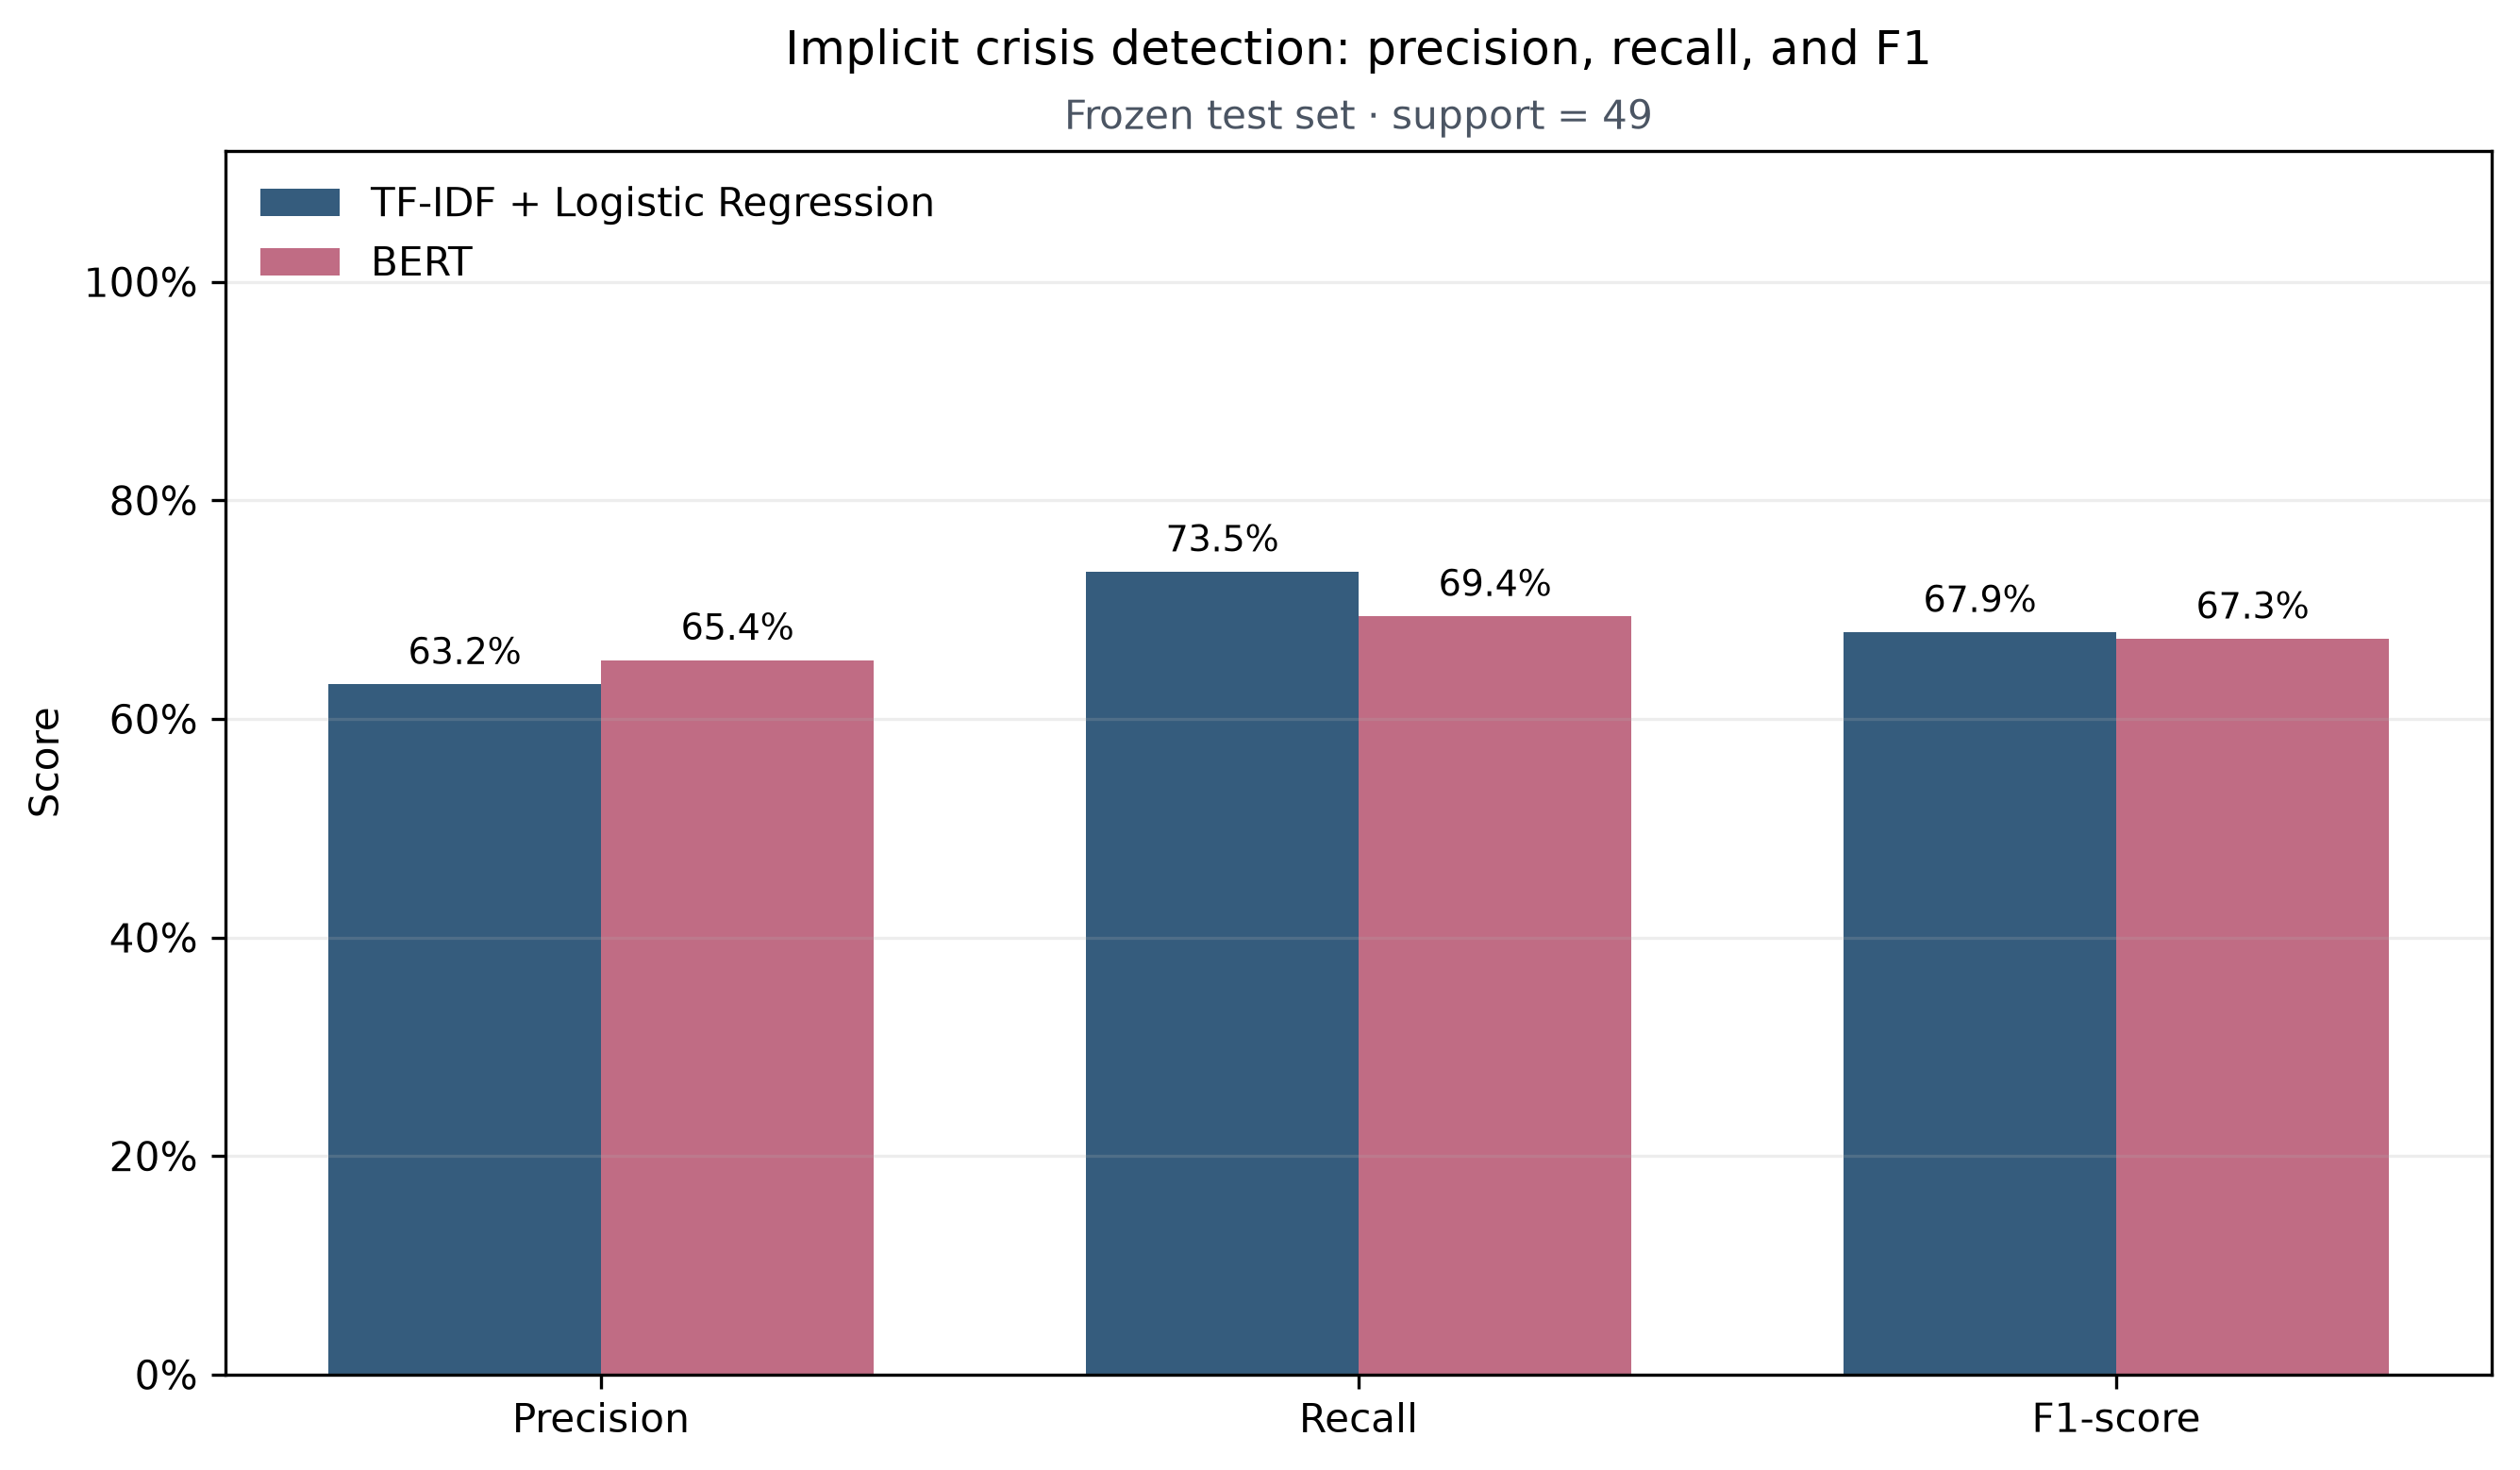
\includegraphics[width=0.7\textwidth]{implicit_crisis_metrics.png}
\caption{Implicit-crisis-specific metric comparison between TF-IDF + Logistic Regression and BERT.}
\end{figure}

\chapter{Example Prediction Outputs}

To avoid reproducing sensitive crisis-related message content, this appendix summarizes prediction outcomes only in aggregate form (see Appendix~C and Section~8.11) rather than quoting individual test-set examples. Readers requiring row-level inspection can consult \texttt{results/\pbrk model\_\pbrk comparison/\pbrk predictions.csv} directly within the repository, which contains the full 195-row prediction table with ground truth, both models' predictions and confidences, correctness flags, and an agreement flag per row.

\chapter{Reproducibility Information}

\begin{itemize}[nosep]
  \item \textbf{Python}: 3.10 or newer.
  \item \textbf{Core requirements}: \texttt{requirements.txt} (pandas, NumPy, PyYAML, scikit-learn, joblib, FastAPI, Uvicorn).
  \item \textbf{ML requirements}: \texttt{requirements-ml.txt} (adds PyTorch, Transformers, Accelerate), installed on top of the core requirements.
  \item \textbf{Artifact retrieval}: \texttt{git lfs pull}, required after cloning to fetch the TF-IDF/LR \texttt{.joblib} files and the BERT weight file.
  \item \textbf{Dataset split paths}: \texttt{data/\pbrk final\_\pbrk datasets/\pbrk splits/\pbrk \{train,validation,test\}.csv}.
  \item \textbf{Evaluation script}: \texttt{scripts/\pbrk evaluate\_\pbrk current\_\pbrk models.py}, writing to \texttt{results/\pbrk model\_\pbrk comparison/\pbrk }.
  \item \textbf{Application startup}:\newline
  \texttt{python -m uvicorn backend.app:app --host 127.0.0.1 --port 8000}\newline
  after which the API and frontend are both served at \texttt{http://127.0.0.1:8000/}.
  \item \textbf{Test set}: \texttt{data/final\_\pbrk datasets/splits/test.csv}, 195 rows, shared identically by both models.
  \item \textbf{Frozen artifacts}:\newline
  \texttt{models/tfidf\_\pbrk logistic\_\pbrk regression/\{tfidf\_\pbrk vectorizer,\newline logistic\_\pbrk regression\}.joblib};\newline
  \texttt{models/bert\_\pbrk no\_\pbrk severity/} (weights, tokenizer, config).
\end{itemize}

This reproducibility information covers inference using the already-frozen artifacts and offline evaluation via the evaluation script; it does not claim that BERT's original fine-tuning run is reproduced from the current repository state.


\end{document}
